\documentclass[preprint]{sigplanconf}

\usepackage{amsmath,amssymb,amsopn,amsthm}
\usepackage[T1]{fontenc}
\usepackage{algorithmic,algorithm}
\usepackage{multirow}
\usepackage{cleveref}
\usepackage{graphicx}
\usepackage[usenames,dvipsnames]{color}

\usepackage{tikz}
\usepackage{pgfplots}

\newcommand\todo[1]{{\color{blue} \footnote{\color{blue} TODO: {#1}}}}
\newcommand\citneeded[1]{{\color{blue} \cite{?}\footnote{\color{blue} citation needed. #1}}}

\newcommand\newterm[1]{{\it #1}}
\newcommand\R{\mathbb{R}}
\newcommand\N{\mathbb{N}}
\newcommand\B{\mathbb{B}}
\newcommand\T{\mathcal{T}}
\renewcommand\S{\mathcal{S}}

\newcommand\lspan[2]{\multicolumn{#1}{@{}l}{#2}}

\begin{document}


\special{papersize=8.5in,11in}
\setlength{\pdfpageheight}{\paperheight}
\setlength{\pdfpagewidth}{\paperwidth}

%\conferenceinfo{CONF 'yy}{Month d--d, 20yy, City, ST, Country} 
%\copyrightyear{20yy} 
%\copyrightdata{978-1-nnnn-nnnn-n/yy/mm} 
%\doi{nnnnnnn.nnnnnnn}

%\titlebanner{banner above paper title}        % These are ignored unless
%\preprintfooter{short description of paper}   % 'preprint' option specified.

\title{Bellmania: Deriving Implementations from Specifications by Transformation}

%\authorinfo{Shachar Itzhaky}
%           {MIT CSAIL}
%           {shachari@mit.edu}
\authorinfo{Double-blind submission}
           {}
           {}

\maketitle

\begin{abstract}
Programmers almost never write optimal code on the first phase.
Instead, they usually begin with a simplified, possibly inefficient, or even
na\"ive implementation. When the result is satisfactory, they would move
on to revise the code in order to improve performance. These normally
change the code considerably compared to the original version. It is especially
true for code that targets multi-core processors, since many considerations
must be taken into account for parallel code in order to utilize all available
cores.

Clearly, each iteration becomes more tedious as the code increases in complexity,
and naturally holds more chance of introducing defects. The programmer must
exercise care to make sure that each version is functionally equivalent to the
previous one. This is when mechanical reasoning can prove useful, by 
(a) packaging familiar techniques as routines, thus avoiding repetitive work, and
(b) checking each modification step, warning the developer when functionality
may be accidentally changed.

We present Bellmania, a framework comprising of a language for specifying
dynamic programming algorithms as recurrences,
and a calculus that facilitates gradual transformation of these 
specifications into efficient implementations.
In particular, it supports using the Divide and Conquer technique to derive
parallel implementations that optimally utilize memory caches.
\end{abstract}

\category{CR-number}{subcategory}{third-level}

\keywords
synthesis, dynamic programming, smt

\section{Introduction}
\label{intro}

\begin{center}$\vdots$\end{center}

As a motivating example, we consider the Simplified Gap problem.
An intelligent agent is given two strings $x$ and $y$, and is requested
to make them equal by deleting the characters at index range $[i..j)$
from $x$, at a cost of $w_{ij}$ ($0\leq i<j\leq |x|$), from $y$,
at a cost of $w'_{ij}$ ($0\leq i<j\leq |y|$), or by repeating these steps
an arbitrary number of times.
\footnote{In the full version of the gap problem, the agent is also allowed to replace a character $\alpha$ with a character $\beta$, at some cost $c_{\alpha\beta}$.}

The optimal cost is given by the following recurrence:

\begin{equation}
\renewcommand\arraystretch{1.5}
\begin{array}{l@{}l}
	G_{ij} ~=~  &
	\begin{cases}
		0                        & i=j=0 \\
		w_{0j}                   & i=0, j>0 \\
		w'_{i0}                  & i>0, j=0 \\
		\begin{array}{@{}l@{~}l}
		  \min\langle & \underset{0\leq q<j}\min ~ G_{iq} + w_{qj}, \\
		              & \underset{0\leq p<i}\min ~ G_{pj} + w'_{pi}~\rangle
		\end{array}              & i,j>0
	\end{cases}
\end{array}
\label{intro:gap spec}
\end{equation}

\smallskip\noindent
where the desired value is $G_{|x||y|}$.

\medskip
With standard dynamic programming, this recurrence can be computed
with an iterative program, by understanding the dependency pattern:
each value $G_{ij}$ is computed from other values $G_{i'j'}$ with lower
indexes, $i'<i$, ~$j'<j$. Therefore, considering $G$ as a two-dimensional
array, it can be filled in a single pass from left to right and from top
to bottom.

\newcommand\FORLINE[1]{\STATE\algorithmicfor~{#1} \algorithmicdo~}

\begin{algorithm}
\renewcommand\arraystretch{1.3}
\begin{algorithmic}
  \STATE $G_{00} := 0$
  \FORLINE{$j=1..|y|$}  $G_{0j} := w_{0j}$  
  \FOR{$i=1..|x|$}
    \STATE $G_{i0} := w'_{i0}$
    \FOR{$j=1..|y|$}
      \STATE $G_{ij} :=
        \begin{array}[t]{@{}l@{~}l} 
          \min\langle & \underset{0\leq q<j}\min ~ G_{iq} + w_{qj}, \\
                      & \underset{0\leq p<i}\min ~ G_{pj} + w'_{pi}~\rangle 
        \end{array}$
    \ENDFOR
  \ENDFOR
\end{algorithmic}
\end{algorithm}

The same intuition underlies the divide-and-conquer approach for making
a parallel version of the same computation. The array $G$ is partitioned into
quadrants and dependencies are observed at the level of quadrants. The same reasoning
has to be repeated at a coarser level;
so, say the quadrants are labeled 1, 2, 3, and 4, then the computations of 2 and 3 depend on 1,
and the computation of 4 depends on 2 and 3.

\newcommand\qbox[1]{\fbox{\scriptsize#1}}

\begin{figure}[b]
$\renewcommand\arraystretch{2}G ~=~
 \begin{array}{|@{\quad}c@{\quad}|@{\quad}c@{\quad}|} \hline 1 & 2 \\[1mm] \hline 3 & 4 \\[1mm] \hline\end{array}$
\qquad
$\begin{array}{l}\qbox1 \rightsquigarrow \qbox2 \\ 
\qbox1 \rightsquigarrow \qbox3 \\ \qbox2\rightsquigarrow \qbox4 \\ \qbox3 \rightsquigarrow \qbox4\end{array}$
\end{figure}

\medskip
The algorithm designer then writes the following pseudo-code:

\begin{algorithmic}[1]
  \STATE Compute \qbox1 (using only input data $w,w'$).
  \STATE Compute \qbox2 using data from \qbox1.
  \STATE Compute \qbox3 using data from \qbox1.
  \STATE Compute \qbox4 using data from \qbox2 and \qbox3.
\end{algorithmic}

We say that the computation is \newterm{stratified},
in the sense that information flows only in one direction. It can be depicted as
a sequence of steps, each of which reads some regions from the array (possibly none)
and writes into a target region. It can be viewed as a chain, like the one in
\Cref{intro:chain}.

\begin{figure}
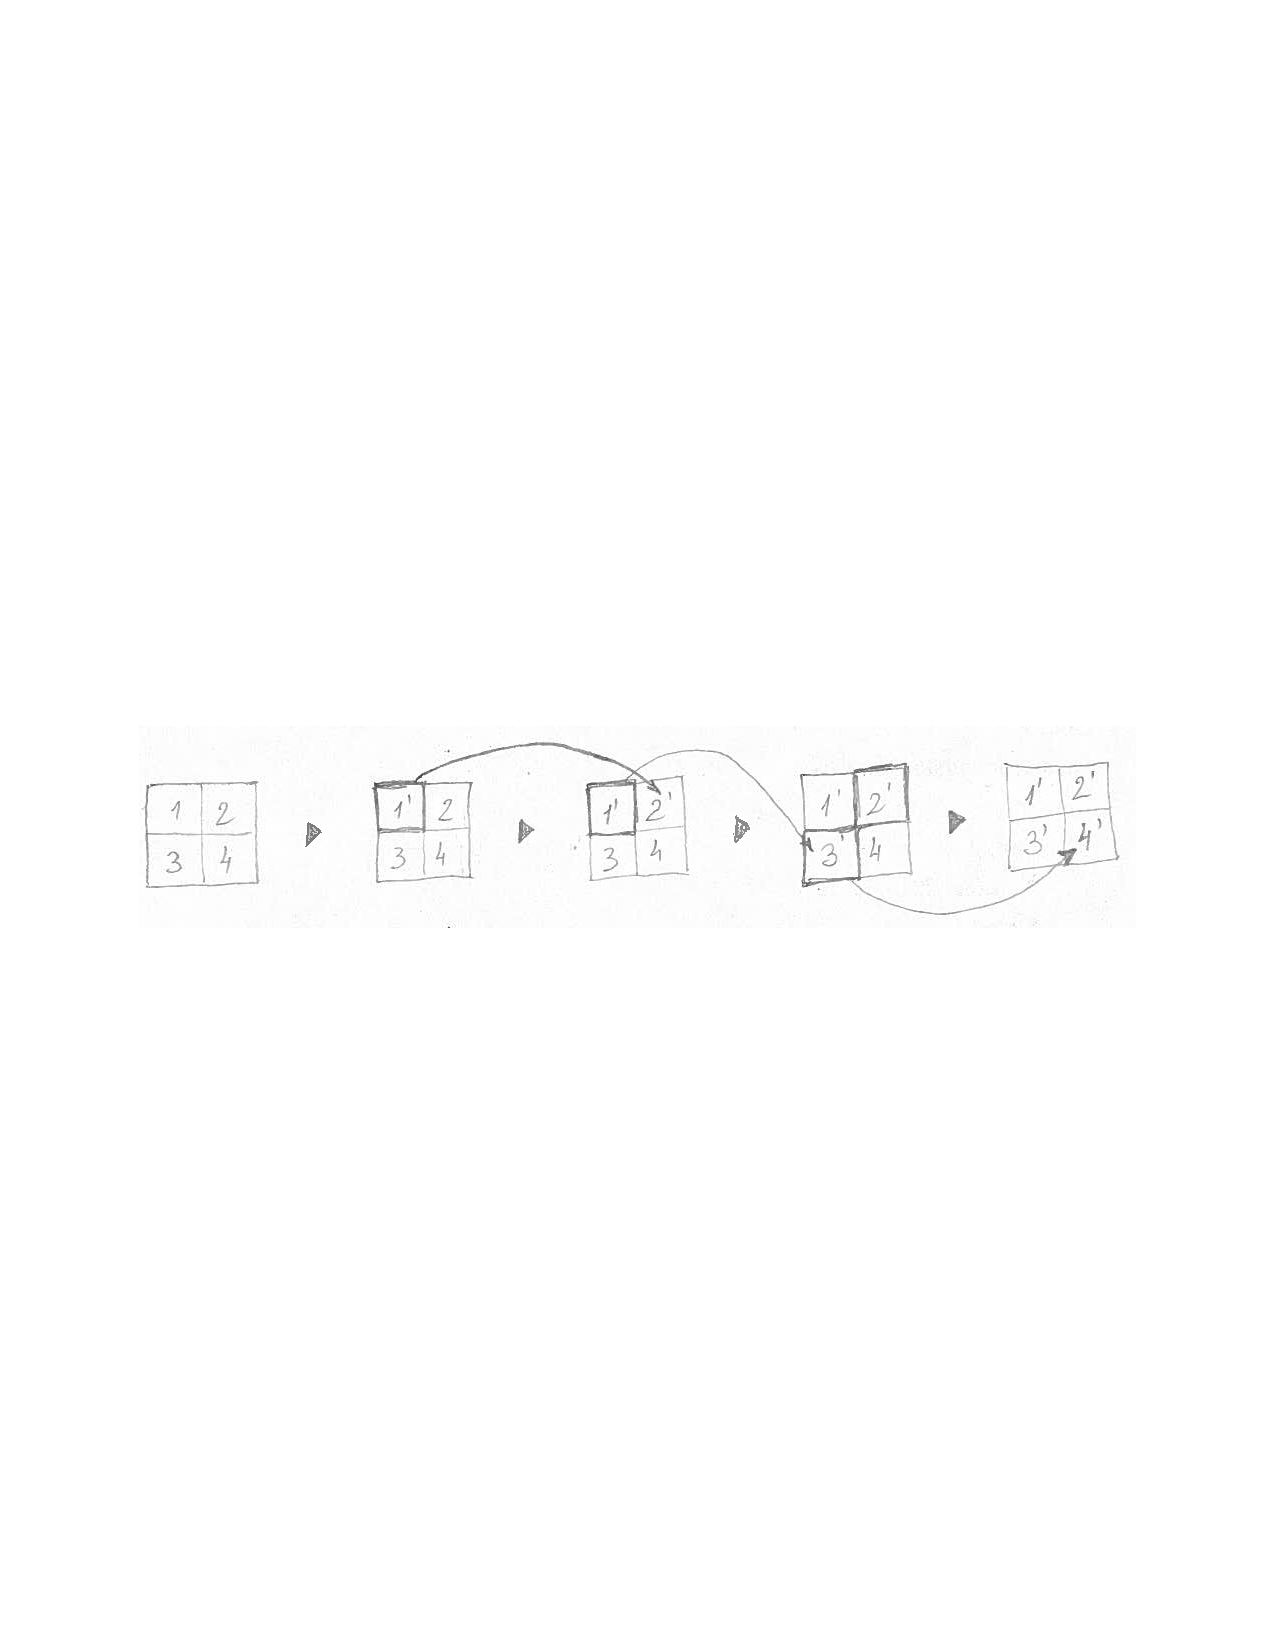
\includegraphics[width=.47\textwidth]{img/gap-stratify1}
\caption[caption]{\label{intro:chain}
  Stratified computation for Simplified Gap. \\[.2em]
  Thick borders indicate the region that is read at each step.}
\end{figure}

At this point it can be noticed that step 1 is equivalent to the original
algorithm when given as input the prefixes of $x$ and $y$ whose length correspond to the
height and width of \qbox1.

With the other three steps, however, things are not so simple:
each of them is required to process some data in addition to the input.
For example, step 2 is required to read values from \qbox1, due to the expression
$G_{iq}$ (where $\scriptstyle 0\leq q<j$).
In order to reason more formally, we define $J$ and $K$ the index sets of the rows
and columns, respectively; $J_0$, $J_1$ for the top and bottom row indexes, respectively;
and $K_0$, $K_1$ for the left and right column indexes (\Cref{intro:slice G}).
The specifications for step 2 then take the following form:

\begin{figure}
\[
\renewcommand\arraystretch{2}
\begin{array}{c|c|c|c|}
  \multicolumn{2}{c}{} & \multicolumn{2}{c}{K} \\ \cline{3-4}
  \multicolumn{2}{c}{} & \multicolumn{1}{c}{K_0}  & \multicolumn{1}{c}{K_1}\\ \cline{3-4}
  \multirow{2}{*}{$J$} & J_0 & 1 & 2 \\ \cline{3-4}
    & J_1 & 3 & 4 \\ \cline{3-4}
\end{array}
\]
\caption{\label{intro:slice G}
  Addressing quadrants in a two-dimensional array.}
\end{figure}

\makeatletter
\newcommand{\LeftEqNo}{\let\veqno\@@leqno}
\makeatother

\begin{equation}\LeftEqNo
\renewcommand\arraystretch{1.5}
\begin{array}{l@{}l}
	G_{\,(i :: J_0)\,(j :: K_1)} ~=~  \\
	\qquad
	\begin{cases}
		0                        & i=j=0 \\
		w_{0j}                   & i=0, j>0 \\
		w'_{i0}                  & i>0, j=0 \\
		\begin{array}{@{}l@{~}l}
		  \min\langle & \underset{0\leq (q::K) <j}\min ~ G_{iq} + w_{qj}, \\
		              & \underset{0\leq (p::J_0) <i}\min ~ G_{pj} + w'_{pi}~\rangle
		\end{array}              & i,j>0
	\end{cases}
\end{array}
\end{equation}

\medskip
Type annotations have been placed on $i$, $j$, $p$, and $q$ to define the regions
over which they range. $i::J_0, j::K_1$ means that the element $G_{ij}$
is always in \qbox2. Similarly, $G_{pj}$ is also in \qbox2. $G_{iq}$ is either in
\qbox1 or in \qbox2.

\begin{figure}
\begin{tabular}{l}
\includegraphics{img/gap-depend}\end{tabular}
\todo{for the simplified version, the cell (i-1,j-1) should not be grayed}
\caption{\label{intro:gap dependency matrix}}
\end{figure}

To address the situation, the algorithm designer would like to separate the parts
of the computation that read from \qbox1 from the parts that read from \qbox2.
This can be achieved here by splitting the $\min_{0\leq(q::K)<j}$ into two
ranges, according to the region in which $G_iq$ resides.

\begin{equation}\LeftEqNo
\renewcommand\arraystretch{1.5}
\begin{array}{l@{}l}
	G_{\,(i :: J_0)\,(j :: K_1)} ~=~  \\
	\qquad
	\begin{cases}
		0                        & i=j=0 \\
		w_{0j}                   & i=0, j>0 \\
		w'_{i0}                  & i>0, j=0 \\
		\begin{array}{@{}l@{~}l}
		  \min\langle & \underset{(q::K_0)}\min ~ G_{iq} + w_{qj}, \\
		              & \underset{(q::K_1) <j}\min ~ G_{iq} + w_{qj}, \\
		              & \underset{0\leq (p::J_0) <i}\min ~ G_{pj} + w'_{pi}~\rangle
		\end{array}              & i,j>0
	\end{cases}
\end{array}
\end{equation}

The path becomes clear: compute $\min_{(q::K_0)} ~ G_{iq} + w_{qj}$ first, for all $i$, $j$
in \qbox2. Then use the results to compute $G_{ij}$.

\begin{equation}\LeftEqNo
\renewcommand\arraystretch{1.5}
\begin{array}{l@{}l}
	G_{\,(i :: J_0)\,(j :: K_1)} ~=~  \\
	\qquad
	\textrm{let}~\psi_{ij} = \underset{(q::K_0)}\min ~ G_{iq} + w_{qj} \\
	\qquad\textrm{in} \\
	\qquad
	\begin{cases}
		0                        & i=j=0 \\
		w_{0j}                   & i=0, j>0 \\
		w'_{i0}                  & i>0, j=0 \\
		\begin{array}{@{}l@{~}l}
		  \min\langle & \psi_{ij}, \\
		              & \underset{(q::K_1) <j}\min ~ G_{iq} + w_{qj}, \\
		              & \underset{0\leq (p::J_0) <i}\min ~ G_{pj} + w'_{pi}~\rangle
		\end{array}              & i,j>0
	\end{cases}
\end{array}
\label{intro:let in 2}
\end{equation}

\medskip
The second part in \eqref{intro:let in 2} starts to look similar to \eqref{intro:gap spec}:
in particular, the types of $p$ and $q$ are the same as those of $i$ and $j$.
In fact, if we set $\psi_{ij}=\infty$, we get \eqref{intro:gap spec} as a special case,
only with $J_0$ and $K_1$ instead of $J$ and $K$.
It therefore makes sense to write a version that generalizes both.

\begin{equation}\LeftEqNo
\renewcommand\arraystretch{1.5}
\begin{array}{l}
	A_{\,\psi\, (i :: J)\, (j :: K)} ~=~  \\
	\qquad
	\begin{cases}
		0                        & i=j=0 \\
		w_{0j}                   & i=0, j>0 \\
		w'_{i0}                  & i>0, j=0 \\
		\begin{array}{@{}l@{~}l}
		  \min\langle & \psi_{ij}, \\
		              & \underset{(q::K)<j}\min ~ A_{\psi iq} + w_{qj}, \\
		              & \underset{(p::J)<i}\min ~ A_{\psi pj} + w'_{pi}~\rangle
		\end{array}              & i,j>0
	\end{cases}
\end{array}
\label{intro:gap phase A}
\end{equation}

\medskip
And we can now rewrite \eqref{intro:gap spec} and \eqref{intro:let in 2} as
%
\begin{equation}
	G_{ij} ~=~ A_{\,(\infty^{JK})\,(i::J)\,(j::K)}
\end{equation}
%
\begin{equation}
\renewcommand\arraystretch{1.3}
\begin{array}{l@{}l}
	G_{\,(i :: J_0)\,(j :: K_1)} ~=~ 
	& \textrm{let}~\psi_{ij} = \underset{(q::K_0)}\min ~ G_{iq} + w_{qj} \\
	& \textrm{in}~A_{\,\psi\,(i::J_0)\,(j::K_1)}
\end{array}	
\label{intro:let in 2 using A}
\end{equation}

\medskip
It takes a bit more insight to notice that \eqref{intro:let in 2 using A} can be further
generalized into:
%
\begin{equation}
\renewcommand\arraystretch{1.5}
\begin{array}{l@{}l}
	A_{\,\psi\,(i :: J)\,(j :: K)} ~=~  \qquad\mbox{(if $i\in J_0$, $j\in K_1$)}\\
	\qquad
	\textrm{let}~\psi'_{ij} = \min \langle~\psi_{ij}, \underset{(q::K_0)}\min ~ G_{iq} + w_{qj}~\rangle \\
	\qquad\textrm{in}~
	A_{\,\psi'\,(i::J_0)\,(j::K_1)}
\end{array}
\label{intro:let in A}
\end{equation}

That is the core of the divide and conquer method: representing the output as a combination
of smaller instances of the problem, or sub-problems, yielding a solution that is essentially
a recursive routine, or a set of mutually recursive routines. In \eqref{intro:let in A}, the
``let''-expression $\psi'_{ij} = \min \langle~\psi_{ij}, \min_{(q::K_0)} ~ G_{iq} + w_{qj}~\rangle$
is another sub-problem that has to be addressed using the same slicing technique.
Once all the pieces fit together, it is possible to cut the space into arbitrarily small pieces,
that fit nicely in each core's local cache. This greately increases performance, as demonstrated
by~\citneeded{perhaps include a table with exact figures}. 

\begin{center}$\vdots$
\end{center}

\subsection{Main Contributions}

\begin{enumerate}
  \item We develop a small set of tactics that can be used to transform a class of recurrence
  specifications intro equivalent divide-and-conquer programs, that admit parallel cache-local
  implementations, in a principled, systematic manner.
  \item We prove that these tactics are semantics-preserving, assuming some side conditions are met
  at the point when the tactic is applied.
  \item We show that the side conditions can be effectively translated into first-order closed
  formulas, and verified automatically by SMT solvers.
\end{enumerate}


\section{A Unified Language}

\newcommand\semp[1]{[\![{#1}]\!]}
\newcommand\fix{\operatorname{fix}}

Bellmania uses the same language for specifications and for programs.  Its core is simply-typed
$\lambda$-calculus with universally quantified type variables (polymorphic types).

We write abstraction terms as $(v:\T)\mapsto e$, where $\T$ is the type of the argument $v$ and $e$ is
the body. Curried functions $(v_1:\T_1)\mapsto (v_2:\T_2) \mapsto \cdots \mapsto (v_n:\T_n) \mapsto e$ are abbreviated 
as $(v_1:\T_1)\cdots(v_n:\T_n)\mapsto e$.

The semantics differ slightly from that of traditional functional languages: arrow types $\T_1\to\T_2$
are interpreted as {\bf mappings} from values of type $\T_1$ to values of type $\T_2$. Algebraically,
interpretations of types, $\semp{\T_1}$, $\semp{\T_2}$, are sets, and interpretations of arrow-typed terms,
$f : \T_1\to\T_2$, are {\bf partial functions} --- $\semp{f} : \semp{T_1}\rightharpoonup\semp{T_2}$.
This implies that a term $t : \T$ may evaluate to an \newterm{undefined} value, $\semp{t}=\bot_\T$
(We would shorten it to $\semp{t}=\bot$ when the type is either insignificant or understood from the context).
For simplicity, we shall identify $\bot_{\T_1\to\T_2}$ with the empty mapping $(v:\T_1)\mapsto\bot_{\T_2}$.

\subsection{Liquid Types}

The core is augmented with predicate abstraction in the form of logically quantified data types 
(Liquid Types~\citneeded{}). These are refinement types restricted via a set of abstraction predicates,
called \newterm{qualifiers}, which are defined over the base types.
Some qualifiers are built-in, and more can defined by the user. To keep the syntax simple, we somewhat
limit the use of qualifiers, allowing only the following forms:

\begin{itemize}
  \item $\{v:\T ~|~ P(v)\}$, abbreviated as $\T\cap P$. When the signature of $P$ is known (which is
  almost always), it is enough to write $P$.
  \item $\{v:\T ~|~ P(v)\land Q(v)\}$, abbreviated as $\T\cap P\cap Q$, or just $P\cap Q$. This extends
  to any number of conjuncts of the same form.
  \item $x : \T_2 \to \{v:\T_2 ~|~ R(x,v)\} \to \T_3$, abbreviated as $\big((\T_1\times\T_2)\cap R\big)\to\T_3$.
  Note that the first parameter to $R$ must be the preceding argument. This extends to quantifiers of
  any arity. Also note that the language does not define tuple types; hence there is no distinction
  between curried and uncurried function types.
\end{itemize}

The type refinement operators $\cap$ and $\times$ may be composed to create conjunctions of qualifiers,
as long as their argument sets are either disjoint or contained, but not overlapping;
for example, \[x:\{v:\T_1~|~P(v)\}\to \{v:\T_2~|~Q(v)\land R(x,v)\}\to\T_3\] can be written as
$\big((P\times Q)\cap R\big)\to\T_3$, but \[x:T_1\to y:\{v:\T_2~|~R(x,v)\} \to \{v:\T_3~|~R(y,v)\}\to\T_4\]
cannot be represented by this restricted fragment.

As with any refinement type system, we define the \newterm{shape} of a type $\T$ to be the raw type
obtained from it by removing all qualifiers.

\subsection{Operators}

\newcommand\applt{\textrm{{\scriptsize\,}\guillemotright{\scriptsize\,}}}

{\color{Gray}
\begin{itemize}
  \item Fixed point operator $\fix f$
  \item Slash operator $/$
  \item Cast operator $t :: \T$ inside expressions (and $t|_{\setlength{\fboxsep}{2pt}\fbox{}}$)
  \item Left application $x \applt f$
\end{itemize}
}

\subsection{Typing Rules}

We define a Bellmania program to be well-typed iff its \newterm{raw form}, obtained by replacing all types by
their shapes, is well-typed. This gives a simple characteristic of type safety without the need to
explictly write any new typing rules. It also means that for $f:\T_1\to\T_2$, $x:T_3$, then $f\,x:\T_2$ whenever
$\T_1$ and $\T_3$ have the same shape. This is much more permissive than the original Liquid Types,
and requires some explanation.\todo{covariance and coercion}

\subsection{Type Inference}

\subsection{Primitives}

The standard library contains some common primitives:

\begin{itemize}
  \item $\R$, a type for real numbers; $\N$ for natural numbers; $\B$ for Boolean true/false.
  \item ${+}, {-} : \forall \T.~\T\to\T\to\T$, polymorphic binary operators.
  \item ${<} : \forall \T. ~\T\to\T\to\B$, a polymorphic order relation.
  \item $\min, \max, \Sigma : \forall \T\,\S.~ (\T\to\S)\to\S$, reduction operators
    on ordered/unordered sequences\todo{bags? multisets?}. The sequence is represented by a mapping $f : \T\to\S$,
    so that e.g. \[\semp{\min f} = \min \{\semp{f}\,v \;|\; v\in\semp{A}, \semp{f}\,v\neq\bot\}\]
    The sequences are expected to be finite.
\end{itemize}

\subsection{Example \hrulefill}
\hrule
\bigskip

\section{Tactics}

A \newterm{tactic} is a scheme of equalities that can be used for rewriting.
When applied to a program term, any occurrence of the left-hand side is replaced by the right-hand side.
A valid application of a tactic is an instance of the scheme that is well-typed and logically valid
(that is, the two sides have the same interpretation in any structure that interprets the free
variables occurring in the equality).

The application of tactics yields a sequence of program terms, each of which is checked to
be equivalent to the previous one. We refer to this sequence by the name \newterm{development}.

We associate with each tactic some \newterm{proof obligations}, listed after the word {\bf Obligations}
in each of the following subsections.
When applying a tactic instance,
these obligations are also instantiated and given to an automated prover. If verified successfully,
they entail the validity of the instance. Clearly the tactic itself can be used as its proof obligation,
if it is easy enough to prove automatically; in such cases we write ``{\bf Obligations:} tactic.''

\newcommand\Obligations{\medskip\noindent{\bf Obligations:} }
\newcommand\reduce{\operatorname{reduce}}
\newcommand\listConcat{{\scriptstyle \,++\,}}

\subsection{Major Tactics}

\subsubsection{Slice} \label{tactics:Slice}
\[f ~=~ f\big|_{X_1} ~\Big/~ f\big|_{X_2} ~\Big/ ~\cdots~ \Big/~ f\big|_{X_r}\]

This tactic partitions a mapping into sub-regions. Each $X_i$ may be a $\times$-expression
according to the arity of $f$.

\Obligations tactic.

Informally, the recombination expression is equal to $f$
when $X_{1..r}$ ``cover'' all the defined points of $f$ (also known as the \newterm{support} of $f$).

\subsubsection{Shrink} \label{tactics:Shrink}
\[f ~=~ f :: \T\]

Used to extra-specify the type of a sub-term.

\Obligations tactic.

For arrow-typed terms, this essentially requires to prove that $f$ is undefined anyway for
argument values outside the domain of $\T$, and that the defined values are in the range of $\T$.

\subsubsection{Stratify} \label{tactics:Stratify}
\[\fix (f\applt g) ~=~ \fix f ~\applt~ \psi\mapsto \fix (\dot\psi\applt g)\]
%
where $\dot\psi$ abbreviates $\theta\mapsto\psi$, with fresh variable $\theta$.

$\psi$ may be fresh, or it may reuse a variable already occurring in $g$, rebinding those occurrences.
The example of this section will illustrate why this is useful.

\Obligations Let $h=f\applt g$ and $g'=\psi\mapsto\dot\psi\applt g$. Let $\theta,\zeta$ be
fresh variables.
\begin{equation}
\renewcommand\arraystretch{1.5}
\begin{array}{l}
f\,(g'\,\zeta\,\theta) ~=~ f\,\zeta \\
g'\,(f\,\theta)\,\theta ~=~ h\,\theta
\end{array}
\label{tactics:Stratify obligations}
\end{equation}

Although the proof is not hard, we defer it to a later theorem.

\subsubsection{Synth} \label{tactics:Synth}
\[\fix\big(h_1 ~\big/~ \cdots ~\big/~ h_r\big) ~=~ 
  (\fix f_1) :: \T_1 ~\big/~ \cdots ~\big/~ (\fix f_r) :: \T_r\]

This tactic is used to generate recursive calls to sub-programs. For $i=1..r$, $f_i$
is typically either $h_i$ or a sub-term occurring earlier in the development.

\Obligations Let $h=h_1/\cdots/h_r$, let $\overline\theta\!=\!\theta_{1..r}$ be $r$ fresh variables, and let
$f = \theta_{1..r} \mapsto (f_1\,\theta_1)::\T_1/\cdots/(f_r\,\theta_r)::\T_r$.
\begin{itemize}
  \item $\T_{1..r}$ are disjoint mappings.
  \item $h\,(f\,\overline\theta) = f\,\overline\theta$.
\end{itemize}

\subsection{Minor Tactics}

\subsubsection{Associativity}
\[\reduce\big\langle \reduce\langle\overline x\rangle, \reduce\langle\overline y\rangle\big\rangle ~=~ \reduce \langle \overline x, \overline y\rangle\]
%
where $\reduce$ is a built-in aggregation ($\min$, $\max$, $\Sigma$), 
and $x$, $y$ are lists of terms (of the same type).

\Obligations none.

\subsubsection{Distributivity}
Let $e$ be an expression with a hole, $e[\square] = (\cdots \square \cdots)$.
%
\[\renewcommand\arraystretch{1.2}
  \begin{array}{@{}r@{~}c@{~}l@{}}
    e[t_1/\cdots/t_r] &=& e[t_1] / \cdots / e[t_r] \\
    e[t_1/\cdots/t_r] &=& \reduce\langle e[t_1],\cdots,e[t_r]\rangle \\
    \reduce e[t_1/\cdots/t_r] &=& \reduce\langle \reduce e[t_1],\cdots,\reduce e[t_r]\rangle
  \end{array}\]

This tactic provides several alternatives for different uses of aggregations.
Clearly, $\big/$ does not distribute over any expression; we give just a few examples
where this tactic is applicable.
\begin{itemize}
  \item $(x/y)+1 ~=~ (x+1)~/~(y+1)$
  \item $x/0 ~=~ \max\langle x,0\rangle$ ~(for $x:\N$)
  \item $\min \big(f\big|_{J_0}~\big/~f\big|_{J_1}\big) ~=~
         \min\left\langle \min f\big|_{J_0} ~,~ \min f\big|_{J_1}\right\rangle$
\end{itemize}

\Obligations tactic.

\subsubsection{Elimination}
\[e[t] ~=~ e[\bot]\]
%
Used to eliminate a sub-term that is either always undefined or has no effect
in the context in which it occurs.

\Obligations tactic.

\subsubsection{Let Insertion}

Let $e$ be an expression with a hole, $e[\square] = (\cdots x_1 \mapsto \cdots x_k\mapsto \cdots \square \cdots)$, 
where $x_{1..k}\mapsto$ are abstraction terms enclosing $\square$. The bodies may contain arbitrary terms
in addition to these abstractions.
%
\[e[t] ~=~ (\overline{x}\mapsto t) ~\applt~ z\mapsto e[z\,\overline{x}]\]
%
where $\overline{x}=x_{1..k}$, and $z$ is either an existing or a fresh variable.

\Obligations tactic, if $z$ occurs free in $e$; otherwise none.

\subsubsection{Padding}
\[t ~=~ \big(t~/~f_1/\cdots/f_r\big) :: \T\]
%
where $\T$ is the type of $t$. This tactic is commonly used with Let insertion,
to make the type of a sub-term match the type of the entire term.

\Obligations tactic.


\subsection{Example \hrulefill}

For simplicity of the example, we assume that the input to the Simplified Gap problem
satisfies triangle inequalities:
%
\begin{equation}
w_{ij} \leq w_{ik} + w_{kj} \qquad w'_{ij} \leq w'_{ik} + w'_{kj}
\label{equ:triangle}
\end{equation}
%
for all (appropriately typed) $i<k<j$.

\medskip
Starting from the specification in \eqref{lang:gap spec}, we apply Synth to turn
$\fix (\theta\,i\,j\mapsto\square/\min\langle\cdots\rangle)$ into $\fix\theta\,i\,j\mapsto\min\langle\square,\cdots\rangle$.
Distributivity and Associativity are used to obtain $f_1$, but the proof is deferred until
Synth is applied so that the prover can use the extra context.

\begin{center}
\fbox{$\begin{array}{l@{}l@{}l}
       \mbox{\underline{Synth}} \\ 
       r=1\\
       h_1=\theta\,i\,j\mapsto{}
	      & \lspan2{0|_{i=0\land j=0} ~\big/~ w'_{0j}|_{i=0} ~\big/~ w_{i0}|_{j=0} ~\big/~} \\
	      & \min\,\langle~ & \min p\mapsto\theta_{pj}+w_{pi}, \\
	      & & \min q\mapsto\theta_{iq}+w'_{qj} ~\rangle \\
       f_1=\theta\,i\,j\mapsto{}
	      & \min\,\langle~ & 0|_{i=0\land j=0} ~\big/~ w'_{0j}|_{i=0} ~\big/~ w_{i0}|_{j=0}, \\
	      & & \min p\mapsto\theta_{pj}+w_{pi}, \\
	      & & \min q\mapsto\theta_{iq}+w'_{qj} ~\rangle
       \end{array}$}
\end{center}

\begin{equation}
  \renewcommand\arraystretch{1.5}
  \begin{array}{@{}l@{}l@{}l@{}}
    G ~=~ \fix \theta\,i\,j\mapsto{}
	      & \min\,\langle~ & 0|_{i=0\land j=0} ~\big/~ w'_{0j}|_{i=0} ~\big/~ w_{i0}|_{j=0}, \\
	      & & \min p\mapsto\theta_{pj}+w_{pi}, \\
	      & & \min q\mapsto\theta_{iq}+w'_{qj} ~\rangle
  \end{array}
\end{equation}

We then apply Let Insertion, followed by Stratify, to obtain the general form of A from \Cref{intro}.

\begin{center}
\fbox{$\begin{array}{l@{}l}
       \mbox{\underline{Let}} \\ 
       e[\square] ~=~ \theta\,i\,j\mapsto\min\langle~ & \square, \\
	      & \min p\mapsto\theta_{pj}+w_{pi}, \\
	      & \min q\mapsto\theta_{iq}+w'_{qj} ~\rangle \\
       \lspan2{~~t ~=~
	      0|_{i=0\land j=0} ~\big/~ w'_{0j}|_{i=0} ~\big/~ w_{i0}|_{j=0}}
       \end{array}$}
\end{center}

\begin{equation}
  \renewcommand\arraystretch{1.5}
  \begin{array}{@{}l@{}l@{}l@{}l@{}}
    G ~=~ & \fix \big(\,& \lspan2{(\theta\,i\,j\mapsto 0|_{i=0\land j=0} ~\big/~ w'_{0j}|_{i=0} ~\big/~ w_{i0}|_{j=0})\applt} \\
	      & & z\,\theta\,i\,j \mapsto \min\,\langle~& z_{\theta ij}, \\
	      & & & \min p\mapsto\theta_{pj}+w_{pi}, \\
	      & & & \min q\mapsto\theta_{iq}+w'_{qj} ~\rangle\,\big)
  \end{array}
\end{equation}

\begin{center}
\fbox{$\begin{array}{l}
       \mbox{\underline{Stratify}} \\ 
       f ~=~ \theta\,i\,j\mapsto 0|_{i=0\land j=0} ~\big/~ w'_{0j}|_{i=0} ~\big/~ w_{i0}|_{j=0} \\
       g ~=~ z\,\theta\,i\,j\mapsto \min\langle z_{\theta ij},\cdots\rangle
       \end{array}$}
\end{center}

\begin{equation}
  \renewcommand\arraystretch{1.5}
  \begin{array}{@{}l@{}l@{}l@{}}
    G ~=~ & \lspan2{\big(\fix \theta\,i\,j\mapsto
	              0|_{i=0\land j=0} ~\big/~ w'_{0j}|_{i=0} ~\big/~ w_{i0}|_{j=0}\big)\applt} \\
	      & \psi\mapsto \fix \theta\,i\,j\mapsto\min\,\langle~ & \psi_{ij} \\
	      & & \min p\mapsto\theta_{pj}+w_{pi}, \\
	      & & \min q\mapsto\theta_{iq}+w'_{qj} ~\rangle
  \end{array}
\end{equation}

\begin{figure}[b]
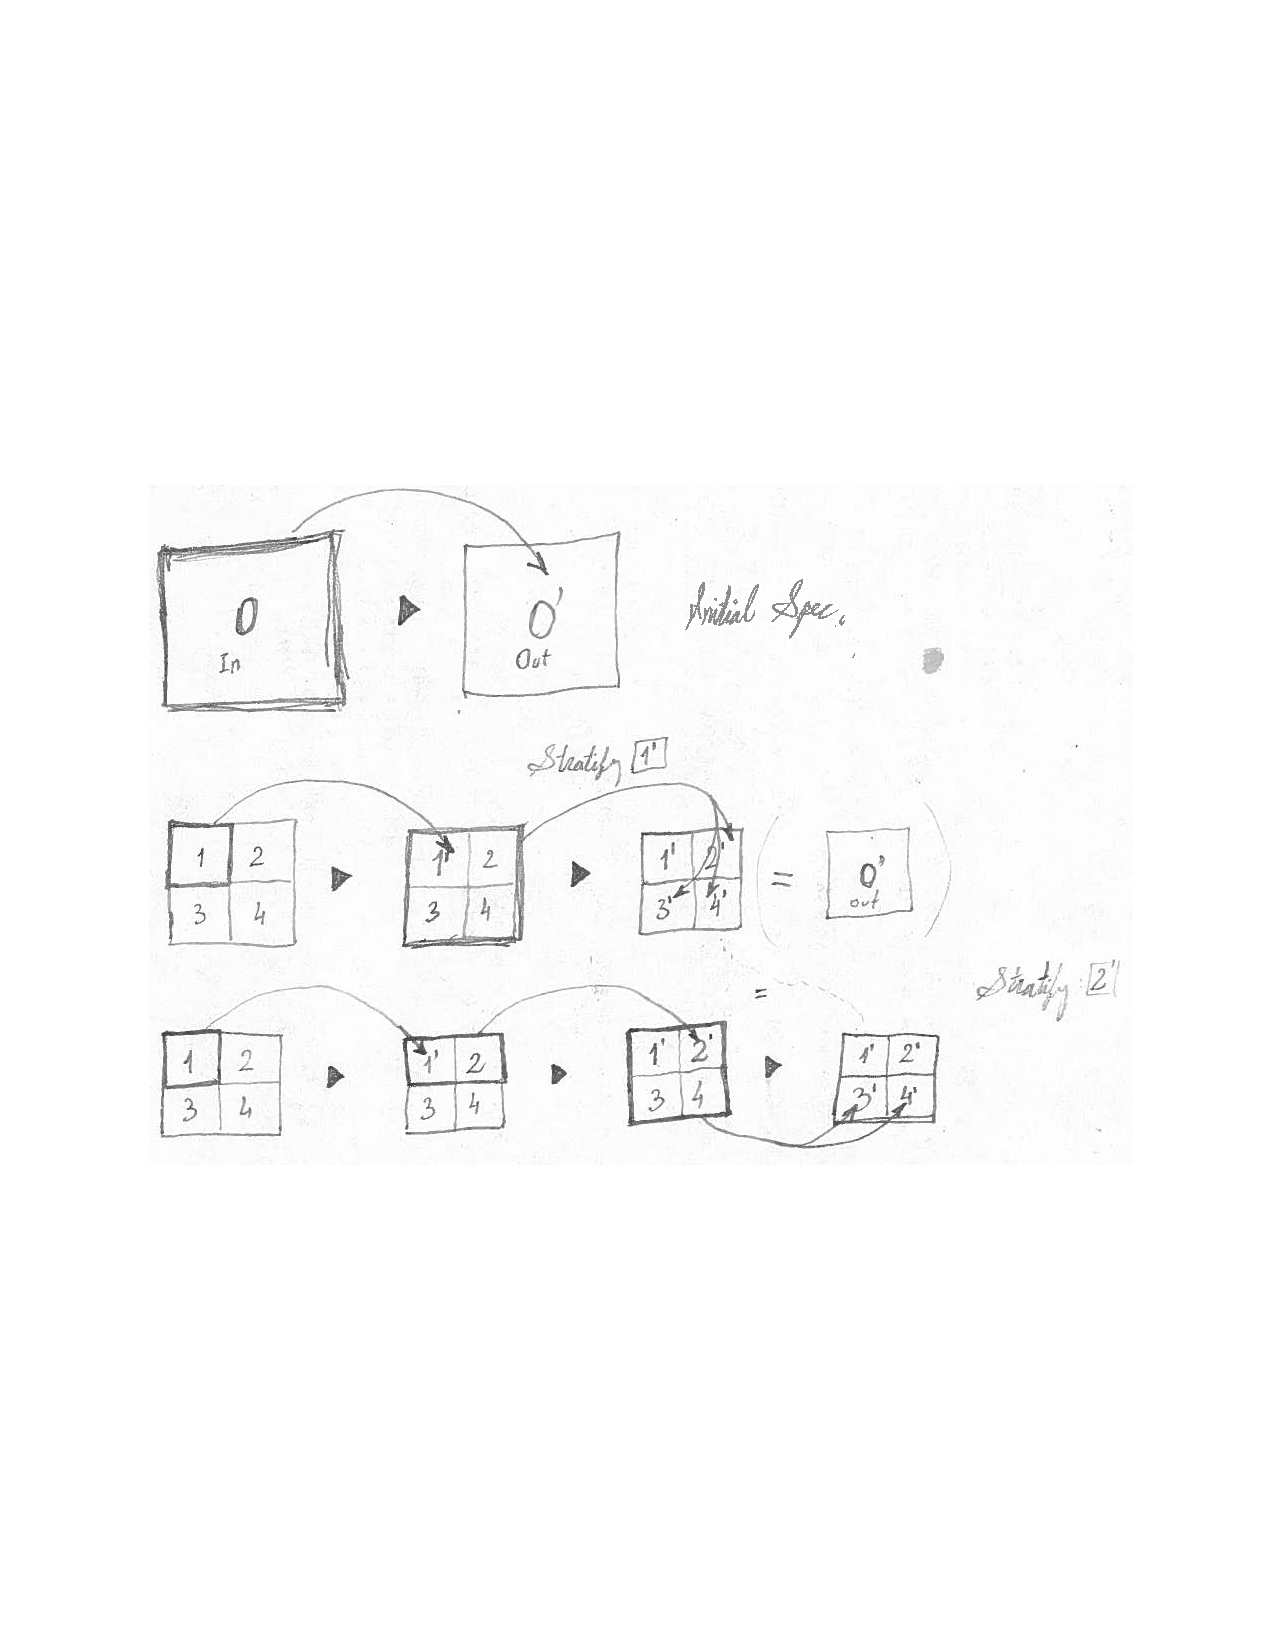
\includegraphics[width=.47\textwidth]{img/gap-stratify2}\\
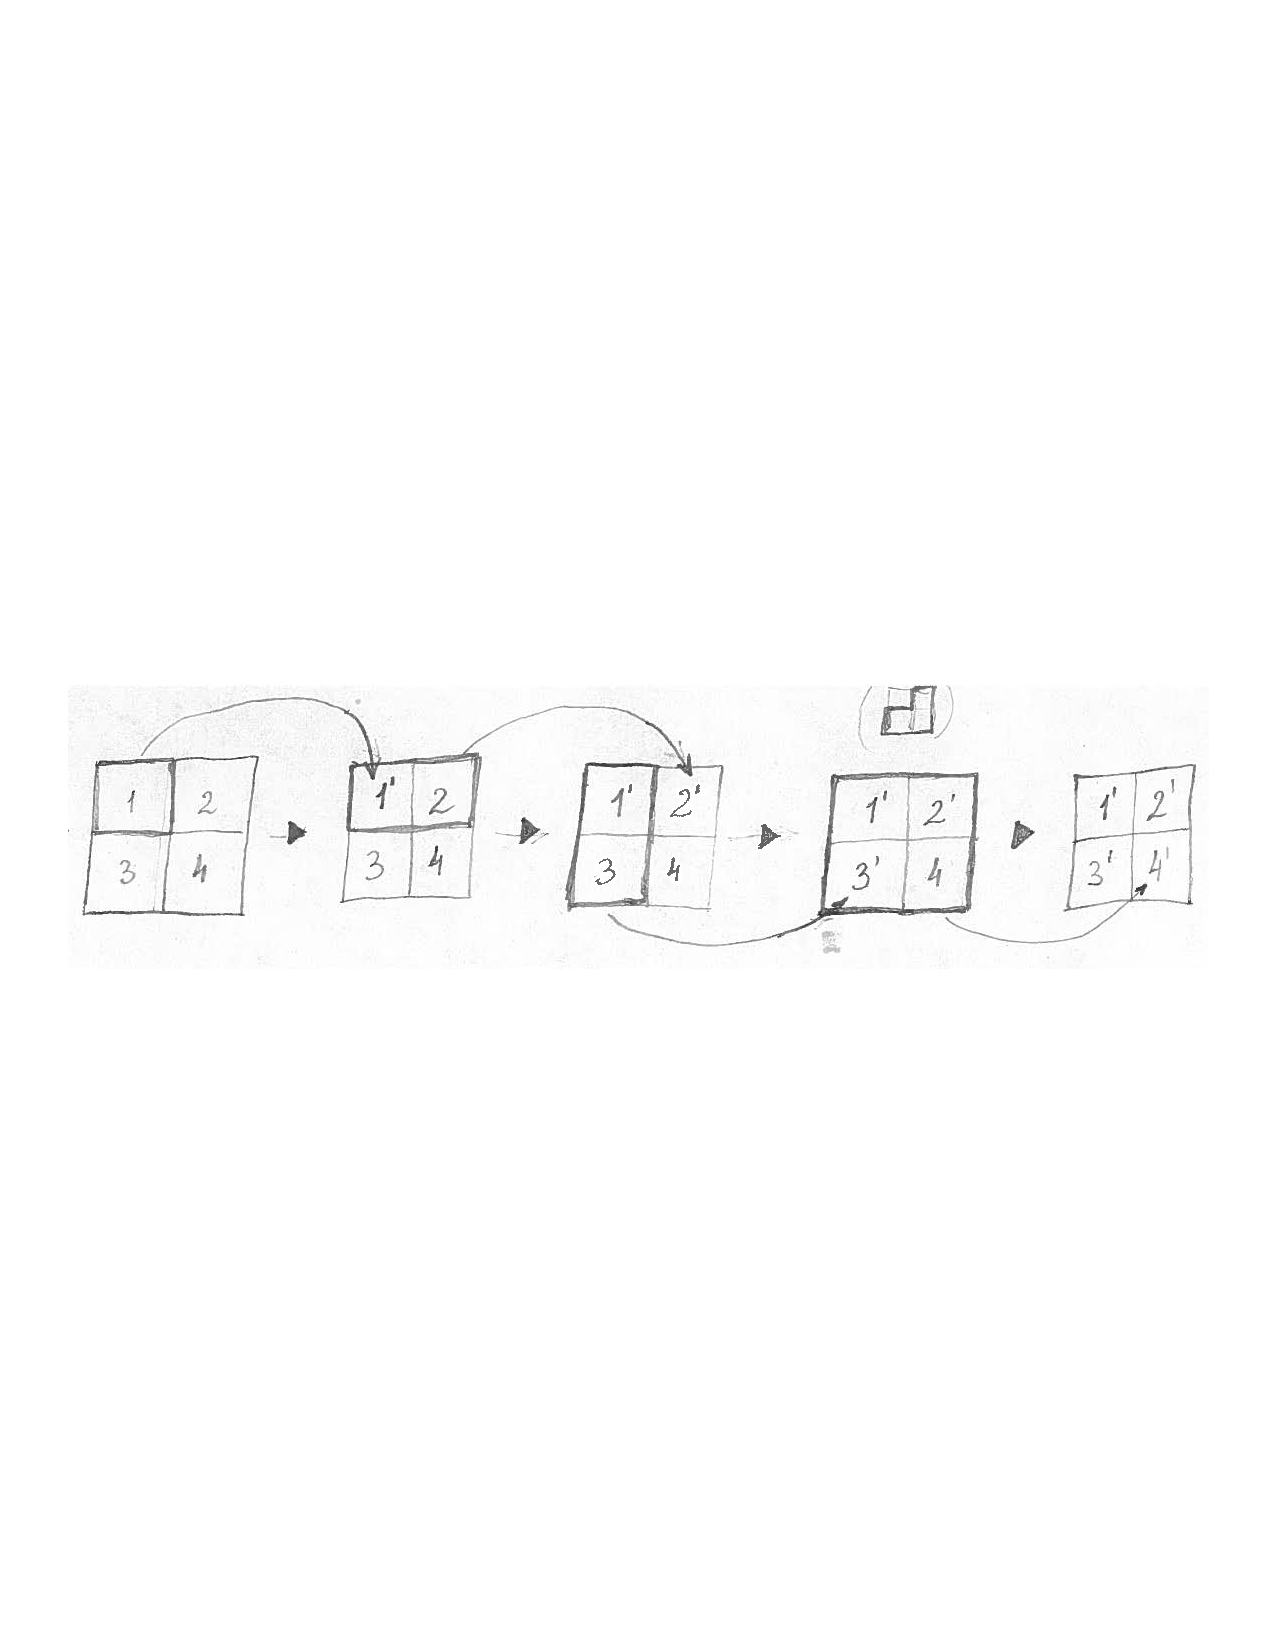
\includegraphics[width=.47\textwidth]{img/gap-stratify3}
\caption{
  Stratification steps for phase ``A'' of Simplified Gap.}
\end{figure}

\hrule
\bigskip


\subsection{Soundness}

\renewenvironment{proof}{\noindent{\bf Proof.~}}{}

\begin{theorem}
Let $s=s'$ be an instance of one of the tactics introduced in this section.
let $a_i=b_i$, $i=1..k$, be the proof obligations. If $\semp{a_i}=\semp{b_i}$
for all interpretations of the free variables of $a_i$ and $b_i$, then
$\semp{s}=\semp{s'}$ for all interpretations of the free variables of $s$ and $s'$.
\end{theorem}

\begin{proof}
For the tactics with {\bf Obligations:} tactic, the theorem is trivial.

\medskip
For Stratify, let $f$, $g$ be partial functions such that
\[\renewcommand\arraystretch{1.3}
  \forall \theta,\zeta.\quad \begin{array}{l}f\,(g\,\zeta\,\theta) ~=~ f\,\zeta \\
  g\,(f\,\theta)\,\theta ~=~ h\,\theta
  \end{array}\quad\]
  
Assume that $\zeta = \fix f$ and $\theta = \fix (g\,\zeta)$. That is,
\[\renewcommand\arraystretch{1.3}
  \begin{array}{l}
    f\,\zeta = \zeta\\
    g\,\zeta\,\theta = \theta
  \end{array}\]
  
Then ---
\[\renewcommand\arraystretch{1.3}
  \begin{array}{l@{}l}
   h\,\theta & {}= g\,(f\,\theta)\,\theta = g\,(f\,(g\,\zeta\,\theta))\,\theta = \\
             & {}= g\,(f\,\zeta)\,\theta = \theta
  \end{array}\]
  
So $\theta = \fix h$. We get $\fix h = \fix \big(g \,(\fix f)\big)$, or, equivalently,
\[\fix h = \fix f \applt \psi\mapsto\fix (g\,\psi)\]

Now instantiate $h$, $f$, and $g$, with $f\applt g$, $f$, and $g'$ from \Cref{tactics:Stratify},
and we obtain the equality in the tactic.

\medskip
For Synth, assume
\[\renewcommand\arraystretch{1.3}
  \forall \overline\theta.\quad h\,(f\,\overline\theta)=f\,\overline\theta \quad\]

And let $\theta=\theta_{1..r}$ such that $\theta_i=\fix f_i$. So $f_i\,\theta_i=\theta_i$.
Let $\theta=\theta_1::\T_1/\cdots/\theta_r::\T_r$.
\[\renewcommand\arraystretch{1.3}
  \begin{array}{l@{}l}
   f\,\overline\theta & {}= (f_1\,\theta_1)::\T_1 / \cdots / (f_r\,\theta_r)::\T_r =  \\
     & {}= \theta_1::\T_1 / \cdots / \theta_r::\T_r = \theta \\[.5em]
   h\,\theta & {}= h\,(f\,\overline\theta) = f\,\overline\theta = \theta
   \end{array}\qquad\]
   
Then $\theta=\fix h$;\\
We get $\fix h = (\fix f_1)::\T_1 / \cdots / (\fix f_r)::\T_r$,
as required.
\end{proof}

\section{Automated Proofs}

This section describes the encoding of proof obligations in first-order logic,
and the ways by which type information is used in discharging them.

Each base type is associated with a sort. The qualifiers are naturally encoded
as predicate symbols with appropriate sorts. In the following paragraphs, we
use a type and its associated sort interchangebly, and the meaning should be clear
from the context.

Each free variable and each node in the formula syntax tree are assigned two
symbols: a function symbol representing the values, and a predicate symbol
representing the support, that is, the set of tuples for which there is a mapping.
For example, a variable $f : J\to\R$ will be assigned a function $f^1: J\to\R$
and a predicate $|f|: J\to\B$. The superscript indictes the function's arity,
and the vertical bars indicate the support.

For refinement-typed symbols, the first-order symbols are still defined in terms
of the shape, and an assumption concerning the support is emitted. For example,
for $g: (J\cap P)\to\R$, the symbols $g^1:J\to\R$, $|g|:J\to\B$ are defined,
with the assumption $\forall \alpha:J.~|g|(\alpha)\limplies P(\alpha)$.

Assumptions are similarly created for nodes of the syntax tree of the formula to
be verified. We define the \newterm{enclosure} of a node to be the ordered set of
all the variables bound by ancestor abstraction nodes ($v\mapsto\ldots$). Since
the interpretation of the node depends on the values of these variables, it is
``skolemized'', i.e., its type is prefixed by the types of enclosing variables.
For example, if $e:\T$, then inside a term $(v:\S)\mapsto \cdots e\cdots$ it would be treated as
type $\S\to\T$.

When a function is being used as an argument in an application term (first-class functions), 
we take its arrow type $\T\to\S$ and create a corresponding \newterm{faux sort} $F_{\T\to\S}$,
an operator $@ : F_{\T\to\S}\to\T\to\S$, and the \newterm{extensionality axiom} ---
\begin{equation}
\forall \alpha\alpha'.~ \big(\forall\beta.~ @(\alpha,\beta)=@(\alpha',\beta)\big)\limplies \alpha=\alpha'
\label{automated:extensionality}
\end{equation}

And for each such function symbol $f^k:\T\to\S$ used as argument, create its 
\newterm{reflection} $f^0:F_{\T\to\S}$ defined by
\begin{equation}
\forall \overline\alpha.~~@(f^0,\overline\alpha)=f^k(\overline\alpha)
\label{automated:reflection}
\end{equation}

Typically, the goal is an equality between functions $f=g$. This naturally translates
to first-order logic as
\[\forall\overline{a}.~\big(|f|(\overline\alpha)\liff|g|(\overline\alpha)\big) \land
  \big(|f|(\overline\alpha) \limplies f^k(\overline\alpha)=g^k(\overline\alpha)\big)\]
  
\subsection{Simplification}

When $f$,$g$ of the goal, $f=g$, are abstraction terms, the above can be simplified by
introducing $k$ fresh variables, $\overline x=x_1\cdots x_k$, and writing the goal as
$f\,\overline x = g\,\overline x$. The types of $\overline x$ are inferred from the types
of $f$ and $g$ (which should have the same shape). We can then apply $\beta$-reduction as
a simplification step. This dramatically reduces the number of quantifiers in the first-order
theory representing the goal, making SMT solving feasible.

Moreover, if the goal has the form $f\,t_1 = f\,t_2$ (e.g. Stratify, \Cref{tactics}) it may
be worth trying to prove that $t_1::\T = t_2::\T$, where $f:\T\to\S$.
This trivially entails the goal and much easier to prove. To understand why
this is a common case, consider \eqref{evaluation:stratify A 1} below: 
notice how $g$ does not modify the quadrant from which $f$ reads.

\section{Case Studies}

In addition to the somewhat artificial Simplified Arbiter,
we tested our technique on two representative problems:
\begin{paragraph}{Gap problem.}
A generalized minimal edit distance problem. Given two input strings 
$\overline{x}=x_1\cdots x_m$ and $\overline{y}=y_1\cdots y_n$,
compute the cost of transforming $x$ into $y$ by any combination of the
following steps
\begin{itemize}
  \item Replacing $x_i$ with $y_j$, at cost $c_{ij}$.
  \item Deleting $x_{p+1}\cdots x_q$, at cost $w_{pq}$.
  \item Inserting $y_{p+1}\cdots y_q$ in $\overline{x}$, at cost $w'_{pq}$.
\end{itemize}

The computation is given by the recurrence \Cref{evaluation:gap spec}.
\end{paragraph}

\begin{paragraph}{Parenthesis problem.} Compute
an optimal placements of parenthesis in a long chain of multiplication, e.g. of matrices, where the input is
are cost functions $x_i$ for accessing the $i$-th element and
$w_{ikj}$ for multiplying elements $[i,k)$ by elements $[k,j)$.
The corresponding recurrence is shown in \Cref{evaluation:paren spec}.
\end{paragraph}

\begin{figure}
\[
  \renewcommand\arraystretch{1.5}
  \begin{array}{@{}l@{}l@{}l@{}}
    \lspan3{w :: ((J\times J)\cap{<})\to\R} \\
    \lspan3{w' :: ((K\times K)\cap{<})\to\R} \\
    G ~=~ \fix \theta\,i\,j\mapsto{}
      & \lspan2{0\big|_{i=0\land j=0} ~\Big/~ w'_{0j}\big|_{i=0} ~\Big/~ w_{i0}\big|_{j=0} ~\Big/~} \\
      & \min~\langle~ & \theta_{(i-1)\,(j-1)} + c_{ij},\\
      & & \min p\mapsto\theta_{pj}+w_{pi}, \\
      & & \min q\mapsto\theta_{iq}+w'_{qj} ~\rangle
  \end{array}
\]
\caption{\label{evaluation:gap spec}
  Specifications for the full version of the Gap DP problem.}
\end{figure}

\begin{figure}
\[
  \renewcommand\arraystretch{1.5}
  \begin{array}{@{}l@{}l@{}l@{}}
    \lspan3{x :: J\to\R} \\
    \lspan3{w :: (J\times J\times J)\to\R} \\
    E ~=~ \fix \theta\,i\,j\mapsto{}
      & \lspan2{x_{ij}\big|_{i+1=j} ~\Big/~} \\
      & \min k\mapsto\theta_{ik}+\theta_{kj}+w_{ikj} \\
  \end{array}
\]
\caption{\label{evaluation:paren spec}
  Specifications for the Parenthesis Assignment DP problem.}
\end{figure}


The next example shows more steps for the Simplified Arbiter test case.


\subsection{Example \hrulefill}

Further developing $A^{IJ}$ \eqref{tactics:arbiter phase A}
we apply Slice to get the four quadrants; $I_0$, $I_1$, $J_0$, $J_1$
(\Cref{intro:quadrants}) are defined as unary qualifiers with the axioms:
\[
\begin{array}{c@{\qquad}c}
  \forall i{:}I.~~I_0(i)\lor I_1(i)   &    \forall i_0{:}I_0,~i_1{:}I_1.~~i_0<i_1 \\
  \forall j{:}J.~~J_0(j)\lor J_1(j)   &    \forall j_0{:}J_0,~j_1{:}J_1.~~j_0<j_1 \\
\end{array}
\]

As a result, the term is
going to grow quite large; to make such terms easy to read and refer to, we provide
boxed letters as labels for sub-terms, using them as abbreviations where they
occur in the larger expression.

\makeatletter
\newcommand{\quadrants@normal}[4]{
  \renewcommand\arraystretch{1.5}
   \begin{array}{c|c}
     #1 & #2 \\ \hline
     #3 & #4
   \end{array}}
\newcommand{\quadrants@small}[4]{
  \renewcommand\arraystretch{0.9}
   \begin{array}{@{~}c@{~}|@{~}c@{~}}
     \scriptstyle #1 & \scriptstyle #2 \\ \hline
     \scriptstyle #3 & \scriptstyle #4
   \end{array}}
\newcommand\quadrants{\@ifstar\quadrants@small\quadrants@normal}
\makeatother

In addition, to allude to the reader's intuition, expressions of the form
$a/b/c/d$ will be written as $\quadrants*{a}{b}{c}{d}$ when the slices
represent quadrants.

\makeatletter
\newcommand{\lbox@small}[1]{ {\setlength{\fboxsep}{1pt}\fbox{\small #1}} }
\newcommand{\lbox@tiny}[1]{ {\setlength{\fboxsep}{1pt}\fbox{\tiny #1}} }
\newcommand\lbox{\@ifstar\lbox@tiny\lbox@small}
\makeatother

\begin{center}
\fbox{$\begin{array}{ll}
       \mbox{\underline{Slice}} \\ 
       f ~=~ \theta\,i\,j\mapsto \cdots \\
       X_1 ~=~ \_\times I_0\times J_0 &
       X_2 ~=~ \_\times I_0\times J_1 \\
       X_3 ~=~ \_\times I_1\times J_0 &
       X_4 ~=~ \_\times I_1\times J_1 \\[.5em]
       \cspan2{\mbox{\small ({\it recall that each} ``\_'' {\it is a fresh type variable})}}
       \end{array}$}
\end{center}

\begin{equation}
  \renewcommand\arraystretch{1.2}
  \begin{array}{@{}r@{}l@{}c@{}c@{}l@{}l@{}}
    A^{^{IJ}} =~ & \lspan5{\psi\mapsto \fix \quadrants{\lbox A}{\lbox B}{\lbox C}{\lbox D}} \\
	\lbox A ~=~ & \theta\,& i & j & \mapsto\min\,\langle~ & \psi_{ij} \\
	      & & ^{^{(I_0)}} & ^{^{(J_0)}} & & \min \vtyped p I \mapsto\theta_{pj}+w_{pij}, \\
	      & & & & & \min \vtyped q J \mapsto\theta_{iq}+w'_{qji} ~\rangle \\
	\lbox B ~=~ & \theta\,& i & j & \mapsto\min\,\langle~ & \psi_{ij} \\
	      & & ^{^{(I_0)}} & ^{^{(J_1)}} & & \min \vtyped p I \mapsto\theta_{pj}+w_{pij}, \\
	      & & & & & \min \vtyped q J \mapsto\theta_{iq}+w'_{qji} ~\rangle \\
	\lbox C ~=~ & \theta\,& i & j & \mapsto\min\,\langle~ & \psi_{ij} \\
	      & & ^{^{(I_1)}} & ^{^{(J_0)}} & & \min \vtyped p I \mapsto\theta_{pj}+w_{pij}, \\
	      & & & & & \min \vtyped q J \mapsto\theta_{iq}+w'_{qji} ~\rangle \\
	\lbox D ~=~ & \theta\,& i & j & \mapsto\min\,\langle~ & \psi_{ij} \\
	      & & ^{^{(I_1)}} & ^{^{(J_1)}} & & \min \vtyped p I \mapsto\theta_{pj}+w_{pij}, \\
	      & & & & & \min \vtyped q J \mapsto\theta_{iq}+w'_{qji} ~\rangle \\
  \end{array}
  \label{tactics:A sliced}
\end{equation}

\begin{tacticbox}{Let}
   e[\square] ~=~ \quadrants*{\square}{\lbox*B}{\lbox*C}{\lbox*D} \qquad
   t ~=~ \lbox A
\end{tacticbox}

\begin{equation}
  A^{^{IJ}} =~ \psi\mapsto \fix \left(\lbox A \applt z\mapsto\quadrants{z}{\lbox B}{\lbox C}{\lbox D}\right)
\end{equation}

\begin{tacticbox}{Stratify[with Padding]}
  \begin{array}{@{} l @{} l @{}}
    f ~=~ \quadrants*{\lbox*A}{\dot\psi}{\dot\psi}{\dot\psi}
         & \mbox{\small ({\it recall that } $\dot\psi=\theta\mapsto\psi$)} \\
    g ~=~ z\mapsto\quadrants*{z}{\lbox*{B}}{\lbox*C}{\lbox*D} &
    \qquad\psi=\psi
  \end{array}
\end{tacticbox}

\begin{equation}
  A^{^{IJ}} =~ \psi\mapsto \fix \quadrants{\lbox A}{\dot\psi}{\dot\psi}{\dot\psi} ~\applt~ \psi\mapsto\fix\quadrants{\dot\psi}{\lbox B}{\lbox C}{\lbox D}
\end{equation}

Notice that an existing variable $\psi$ is reused, rebinding any occurrences within $\lbox B$, $\lbox C$, $\lbox D$.
This effect is useful, as it limits the context of the expression: the inner $\psi$ shadows the outer $\psi$,
meaning $\lbox B$, $\lbox C$, $\lbox D$ do not need to access the data that was input to $\lbox A$, only its
output.

\medskip
The sequence Let, Stratify[with Padding] is now applied in the same manner to $\lbox B$
and $\lbox C$. We do not list the applications as they are analogous to the previous ones.

\begin{equation}
  \renewcommand\arraystretch{1.5}
  \begin{array}{l@{}l}
    A^{^{IJ}} =~ \psi\mapsto{} & \fix \quadrants{\lbox A}{\dot\psi}{\dot\psi}{\dot\psi} ~\applt~ 
                 \psi\mapsto\fix\quadrants{\dot\psi}{\lbox B}{\dot\psi}{\dot\psi} ~\applt \\
               & \psi\mapsto\fix\quadrants{\dot\psi}{\dot\psi}{\lbox C}{\dot\psi} ~\applt~
                 \psi\mapsto\fix\quadrants{\dot\psi}{\dot\psi}{\dot\psi}{\lbox D}
  \end{array}
\end{equation}

\begin{figure}
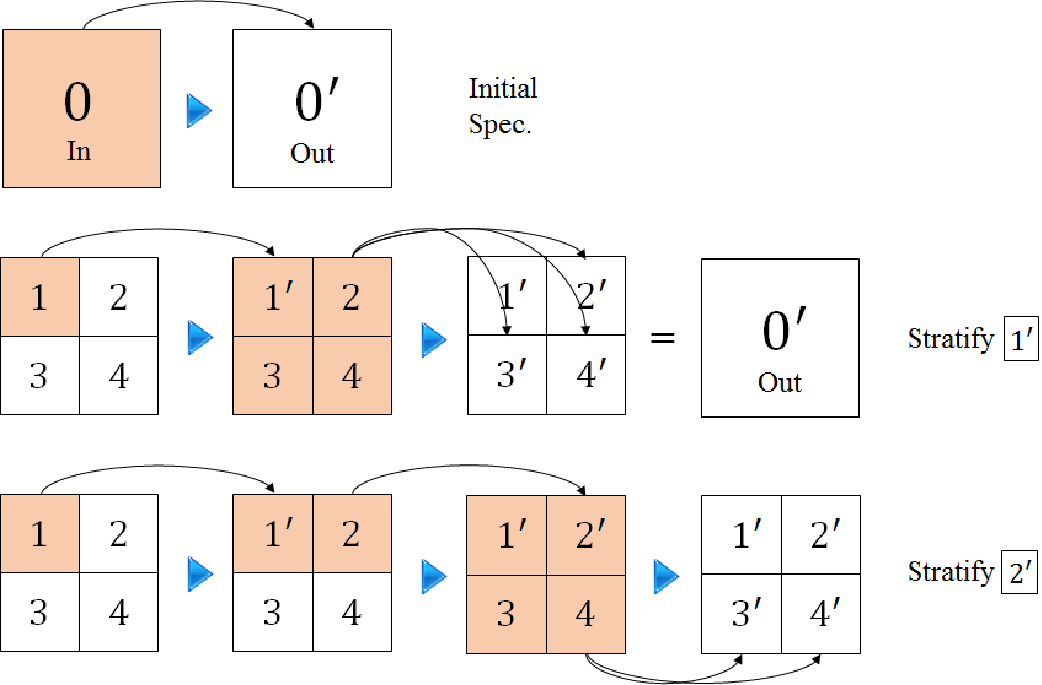
\includegraphics[width=.47\textwidth]{img/arbiter-stratify2}\\
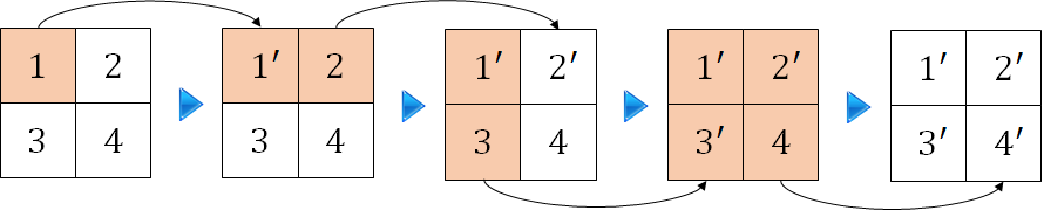
\includegraphics[width=.47\textwidth]{img/arbiter-stratify3}
\caption{
  Stratification steps for phase ``A'' of Simplified Arbiter.}
\end{figure}

\begin{tacticbox}{Synth}
	\begin{array}{@{}l@{}c@{}c@{}l@{}l}
       \lspan5{h_1= \lbox A} \\
       \lspan5{h_{2,3,4}=\dot\psi} \\
	   f_1 = \theta\,& i & j & \mapsto\min\,\langle~ & \psi_{ij} \\
	      & ^{^{(I_0)}} & ^{^{(J_0)}} & & \min \vtyped p {I_0} \mapsto\theta_{pj}+w_{pij}, \\
	      & & & & \min \vtyped q {J_0} \mapsto\theta_{iq}+w'_{qji} ~\rangle \\
	   \lspan5{f_{2,3,4} = \dot\psi}
   \end{array}
\end{tacticbox}

\begin{equation}
  \renewcommand\arraystretch{1.5}
  \begin{array}{l@{}l}
    A^{^{IJ}} =~ \psi\mapsto{} & \quadrants{A^{^{I_0J_0}}_\psi\!\!\!}{\psi}{\psi}{\psi} ~\applt~ 
                 \psi\mapsto\fix\quadrants{\dot\psi}{\lbox B}{\dot\psi}{\dot\psi} ~\applt \\
               & \psi\mapsto\fix\quadrants{\dot\psi}{\dot\psi}{\lbox C}{\dot\psi} ~\applt~
                 \psi\mapsto\fix\quadrants{\dot\psi}{\dot\psi}{\dot\psi}{\lbox D}
  \end{array}
  \label{fix A}
\end{equation}

We note that $\fix f_1=A^{^{I_0J_0}}$ are {\bf identical} terms. Also, we took the liberty
to simplify $\fix\dot\psi$ into $\psi$ --- although this is not necessary --- just to display
a shorter term.

\medskip
The next few tactics will focus on the subterm $\lbox B$ from \eqref{tactics:A sliced}.

\begin{equation}
  \renewcommand\arraystretch{1.2}
  \begin{array}{@{}r@{}l@{}c@{}c@{}l@{}l@{}}
	\lbox B ~=~ & \theta\,& i & j & \mapsto\min\,\langle~ & \psi_{ij} \\
	      & & ^{^{(I_0)}} & ^{^{(J_1)}} & & \min \vtyped p I \mapsto\theta_{pj}+w_{pij}, \\
	      & & & & & \min \vtyped q J \mapsto\theta_{iq}+w'_{qji} ~\rangle
  \end{array}
\end{equation}

\begin{tacticbox}{Slice}
  \begin{array}{@{} l @{}}
    f = \min \vtyped q J \mapsto \theta_{iq}+w'_{qji} \\
    X_1 = J_0\to\_ \qquad X_2 = J_1\to\_
  \end{array}
\end{tacticbox}

\begin{equation}
  \renewcommand\arraystretch{1.2}
  \begin{array}{@{}r@{}l@{}c@{}c@{}l@{}l@{}l@{}}
	\lbox B ~=~ & \theta\,& i & j & \mapsto\min\,\big\langle~ & \psi_{ij} \\
	      & & ^{^{(I_0)}} & ^{^{(J_1)}} & & \lspan2{\min \vtyped p I \mapsto\theta_{pj}+w_{pij},} \\
	      & & & & & \min \big( & (\vtyped q {J_0} \mapsto\theta_{iq}+w'_{qji}) ~\big/~ \\
	      & & & & & & (\vtyped q {J_1} \mapsto\theta_{iq}+w'_{qji})\big)  ~\big\rangle
  \end{array}
\end{equation}

\begin{tacticbox}{Distributivity}
  \begin{array}{@{} l @{}}
    e[\square] = \min\square \\
    t_1 = \min \vtyped q {J_0} \mapsto \theta_{iq}+w'_{qji} \\
    t_2 = \min \vtyped q {J_1} \mapsto \theta_{iq}+w'_{qji} \\
  \end{array}
\end{tacticbox}

\begin{tacticbox}{Associativity}
  \begin{array}{@{} l @{} l @{}}
    \lspan2{\reduce = \min} \\
    \overline x_1 ={} & \psi_{ij} \\
    \overline x_2 ={} & \min \vtyped p I \mapsto\theta_{pj}+w_{pij} \\
    \overline x_3 ={} & \min \vtyped q {J_0} \mapsto \theta_{iq}+w'_{qji} ~, \\
                      & \min \vtyped q {J_1} \mapsto \theta_{iq}+w'_{qji}
  \end{array}
\end{tacticbox}

\begin{equation}
  \renewcommand\arraystretch{1.2}
  \begin{array}{@{}r@{}l@{}c@{}c@{}l@{}l@{}}
	\lbox B ~=~ & \theta\,& i & j & \mapsto\min\,\big\langle~ & \psi_{ij} \\
	      & & ^{^{(I_0)}} & ^{^{(J_1)}} & & \min \vtyped p I \mapsto\theta_{pj}+w_{pij}, \\
	      & & & & & \min \vtyped q {J_0} \mapsto\theta_{iq}+w'_{qji}, \\
	      & & & & & \min \vtyped q {J_1} \mapsto\theta_{iq}+w'_{qji} ~\big\rangle
  \end{array}
\end{equation}

\begin{tacticbox}{Let[$\reduce$]}
  \begin{array}{@{} r @{} l @{}}
    e[\square] ={} & \quadrants{\dot\psi}{\theta\,i\,j\mapsto\square}{\dot\psi}{\dot\psi} \\
    \overline a ={} & \psi_{ij}, ~\min \vtyped q{J_0}\mapsto \theta_{iq}+w'_{qji} \\
    \overline b ={} & \min \vtyped p I \mapsto\theta_{pj}+w_{pij}, \\
                    & \min \vtyped q {J_1} \mapsto\theta_{iq}+w'_{qji}
  \end{array}
\end{tacticbox}

\begin{equation}
  \renewcommand\arraystretch{1.2}
  \begin{array}{r @{} l @{} c @{} c @{} l @{} l}
    \lspan6{
    \quadrants{\dot\psi}{\lbox B}{\dot\psi}{\dot\psi} =
      \fix\left(\lbox E \applt z\mapsto\quadrants{\dot\psi}{\lbox F}{\dot\psi}{\dot\psi}\right) 
    } \\[1.5em]
    ~\lbox E ={} &
      \theta & i & j & \mapsto\min\langle & \psi_{ij}, \\
             & & ^{^{(I_0)}} & ^{^{(J_1)}} &
                                          & \min \vtyped q{J_0}\mapsto\theta_{iq}+w'_{qji} \rangle \\
    ~\lbox F ={} &
      \theta & i & j & \mapsto\min\langle & z_{\theta ij}, \\
             & & ^{^{(I_0)}} & ^{^{(J_1)}} &
                                         & \min \vtyped p I \mapsto\theta_{pj}+w_{pij}, \\
             & & & &                     & \min \vtyped q {J_1} \mapsto\theta_{iq}+w'_{qji}\rangle
  \end{array}
\end{equation}

\begin{tacticbox}{Stratify[with Padding]}
  \begin{array}{@{} l @{}}
    f ~=~ \quadrants*{\dot\psi}{\lbox*E}{\dot\psi}{\dot\psi} \\
    g ~=~ z\mapsto\quadrants*{\dot\psi}{\lbox*F}{\dot\psi}{\dot\psi}
    \qquad\psi=\psi
  \end{array}
\end{tacticbox}

\begin{equation}
  \renewcommand\arraystretch{1.2}
  \begin{array}{r @{} l @{} c @{} c @{} l @{} l}
    \lspan6{
    \fix\quadrants{\dot\psi}{\lbox B}{\dot\psi}{\dot\psi} =
      \fix\quadrants{\dot\psi}{\lbox E}{\dot\psi}{\dot\psi} \applt
      \psi\mapsto\fix\quadrants{\dot\psi}{\lbox F}{\dot\psi}{\dot\psi}
    } \\[1.5em]
    ~\lbox E ={} &
      \theta & i & j & \mapsto\min\langle & \psi_{ij}, \\
             & & ^{^{(I_0)}} & ^{^{(J_1)}} &
                                          & \min \vtyped q{J_0}\mapsto\theta_{iq}+w'_{qji} \rangle \\
    ~\lbox F ={} &
      \theta & i & j & \mapsto\min\langle & \psi_{ij}, \\
             & & ^{^{(I_0)}} & ^{^{(J_1)}} &
                                          & \min \vtyped p I \mapsto\theta_{pj}+w_{pij}, \\
             & & & &                      & \min \vtyped q {J_1} \mapsto\theta_{iq}+w'_{qji}\rangle
  \end{array}
\end{equation}

\noindent
Define
\begin{equation}
  \renewcommand\arraystretch{1.2}
  \begin{array}{@{}l @{} l @{\!} c @{} c @{} l @{} l@{}}
  B^{^{IJ_0J_1}} =~ & \psi\mapsto \\
      & \fix
      \theta & i & j & \mapsto\min\langle & \psi_{ij}, \\
           & & ^{^{(I)}} & ^{^{(J_1)}} &
                                          & \min \vtyped q{J_0}\mapsto\theta_{iq}+w'_{qji} \rangle
  \end{array}
\end{equation}

\begin{tacticbox}{Synth}
  \begin{array}{@{} l @{} c @{} c @{} l @{} l @{}}
    \lspan5{h_2 = \lbox E} \\
    \lspan5{h_{1,3,4} = \dot\psi} \\
    f_2 = 
      \theta & i & j & \mapsto\min\langle & \psi_{ij}, \\
             & ^{^{(I_0)}} & ^{^{(J_1)}} &
                                          & \min \vtyped q {J_0} \mapsto\theta_{iq}+w'_{qji}\rangle \\
    \lspan5{f_{1,3,4} = \dot\psi}
  \end{array}
\end{tacticbox}

\begin{tacticbox}{Synth}
  \begin{array}{@{} l @{} c @{} c @{} l @{} l @{}}
    \lspan5{h_2 = \lbox F} \\
    \lspan5{h_{1,3,4} = \dot\psi} \\
    f_2 = 
      \theta & i & j & \mapsto\min\langle & \psi_{ij}, \\
             & ^{^{(I_0)}} & ^{^{(J_1)}} &
                                          & \min \vtyped p {I_0} \mapsto\theta_{pj}+w_{pij}, \\
             & & &                        & \min \vtyped q {J_1} \mapsto\theta_{iq}+w'_{qji}\rangle \\
    \lspan5{f_{1,3,4} = \dot\psi}
  \end{array}
\end{tacticbox}

\begin{equation}
  \fix\quadrants{\dot\psi}{\lbox B}{\dot\psi}{\dot\psi} ~=~
    \quadrants{\psi}{B^{^{I_0J_0J_1}}_\psi\!\!\!\!}{\psi}{\psi} ~\applt~
    \psi\mapsto\quadrants{\psi}{A^{^{I_0J_1}}_\psi\!\!\!}{\psi}{\psi}
  \label{fix B}
\end{equation}

\medskip\noindent
In a similar manner, we will obtain the following:

\begin{equation}
  \fix\quadrants{\dot\psi}{\dot\psi}{\lbox C}{\dot\psi} ~=~
    \quadrants{\psi}{\psi}{C^{^{I_0I_1J_0}}_\psi\!\!\!\!}{\psi} ~\applt~
    \psi\mapsto\quadrants{\psi}{\psi}{A^{^{I_1J_0}}_\psi\!\!\!}{\psi}
  \label{fix C}
\end{equation}

\begin{equation}
  \renewcommand\arraystretch{1.2}
  \begin{array}{@{}l @{} l @{\!} c @{} c @{} l @{} l@{}}
  C^{^{I_0I_1J}} =~ & \psi\mapsto \\
      & \fix
      \theta & i & j & \mapsto\min\langle & \psi_{ij}, \\
           & & ^{^{(I_1)}} & ^{^{(J)}} &
                                          & \min \vtyped p {I_0} \mapsto\theta_{pj}+w_{pij} \rangle
  \end{array}
\end{equation}

\medskip\noindent
And\coa{Do we want to expand these?} ---

\begin{equation}
  \begin{array}{@{} l @{} l @{}}
    \fix\quadrants{\dot\psi}{\dot\psi}{\dot\psi}{\lbox D} ~=~ &
      \quadrants{\psi}{\psi}{\psi}{B^{^{I_1J_0J_1}}_\psi\!\!\!\!} ~\applt~
      \psi\mapsto\quadrants{\psi}{\psi}{\psi}{C^{^{I_0I_1J_1}}_\psi\!\!\!} \\
    &
       ~\applt~ \psi\mapsto\quadrants{\psi}{\psi}{\psi}{A^{^{I_1J_1}}_\psi\!\!\!}
  \end{array}
  \label{fix D}
\end{equation}

This gives the stratified version as shown in \Cref{evaluation:arbiter stratify A chain}.
The read and write regions are already encoded in the types of $A$, $B$, $C$ in 
\eqref{fix A}, \eqref{fix B}, \eqref{fix C}, and \eqref{fix D}.

\medskip
\hrule
\bigskip

We finish this section by presenting some numbers: \Cref{evaluation:solving time}
shows measurements done using two SMT solvers, Z3 and CVC4, and a sample set of tactic
applications used in the derivation of Gap and Parenthesis divide-and-conquer DP implementations.

\begin{table}
\centering
\renewcommand\a{({\it i})}    % relax! it's only for this figure
\renewcommand\b{({\it ii})}
\renewcommand\c{({\it iii})}
\begin{tabular}{|l@{\,}c@{\,}|rr|}
  \cline{3-4}
  \multicolumn{2}{c|}{} & \multicolumn{2}{c|}{\small Solving time ({\it s})} \\
  \multicolumn{2}{c|}{} & \multicolumn{1}{c|}{~Z3~} & \multicolumn{1}{c|}{CVC4} \\
  \hline
  {\bf \hspace{-.1cm}Gap} & &  & \\
  \hline
  Synth                                   &    & T/O & 2.8 \\
  Stratify \qbox1                         &    & 6.2 & 5.8 \\
  Stratify \qbox2                         &    & 3.5 & 0.5 \\
  Let[$\reduce$] + Stratify in \qbox2     &    & 3.1 & 1.9 \\
  Let[$\reduce$] + Stratify in \qbox4     & \a &  10 & 3.9 \\
                                          & \b & 5.7 & 4.7 \\
                                          & \c & 4.7 & 4.3 \\
  \hline
  {\bf \hspace{-.1cm}Parenthesis} & & & \\
  \hline
  Stratify \!\lbox{$\diagdown$}           &    & 0.4 & 0.1 \\
  Stratify \qbox1                         &    & 1.8 & 2.5 \\
  Stratify \qbox2                         &    & 1.7 & 0.6 \\
  \hline
\end{tabular}
\caption{\label{evaluation:solving time}
  Proof search time for proof obligations in a few sample tactic applications.}
\end{table}


\begin{comment}
\subsection{old stuff}


At this point it can be noticed that step 1 is equivalent to the original
algorithm when given as input the prefixes of $x$ and $y$ whose length correspond to the
height and width of \qbox1.

With the other three steps, however, things are not so simple:
each of them is required to process some data in addition to the input.
For example, step 2 is required to read values from \qbox1, due to the expression
$G_{iq}$ (where $\scriptstyle 0\leq q<j$).
In order to reason more formally, we define $J$ and $K$ the index sets of the rows
and columns, respectively; $J_0$, $J_1$ for the top and bottom row indexes, respectively;
and $K_0$, $K_1$ for the left and right column indexes (\Cref{intro:quadrants}).
The specifications for step 2 then take the following form:

\begin{equation}\LeftEqNo
\renewcommand\arraystretch{1.5}
\begin{array}{l@{}l}
	G_{\,(i : J_0)\,(j : K_1)} ~=~  \\
	\qquad
	\begin{cases}
		0                        & i=j=0 \\
		w'_{0j0}                 & i=0, j>0 \\
		w_{0i0}                  & i>0, j=0 \\
		\begin{array}{@{}l@{~}l}
		  \min\langle & \underset{0\leq (q:K) <j}\min ~ G_{iq} + w'_{qji}, \\
		              & \underset{0\leq (p:J_0) <i}\min ~ G_{pj} + w_{pij}~\rangle
		\end{array}              & i,j>0
	\end{cases}
\end{array}
\end{equation}

\medskip
Type annotations have been placed on $i$, $j$, $p$, and $q$ to define the regions
over which they range. $i:J_0, j:K_1$ means that the element $G_{ij}$
is always in \qbox2. Similarly, $G_{pj}$ is also in \qbox2. $G_{iq}$ is either in
\qbox1 or in \qbox2.


To address the situation, the algorithm designer would like to separate the parts
of the computation that read from \qbox1 from the parts that read from \qbox2.
This can be achieved here by splitting the $\min_{0\leq(q:K)<j}$ into two
ranges, according to the region in which $G_{iq}$ resides.

\begin{equation}\LeftEqNo
\renewcommand\arraystretch{1.5}
\begin{array}{l@{}l}
	G_{\,(i : J_0)\,(j : K_1)} ~=~  \\
	\qquad
	\begin{cases}
		0                        & i=j=0 \\
		w'_{0j0}                 & i=0, j>0 \\
		w_{0i0}                  & i>0, j=0 \\
		\begin{array}{@{}l@{~}l}
		  \min\langle & \underset{(q:K_0)}\min ~ G_{iq} + w'_{qji}, \\
		              & \underset{(q:K_1) <j}\min ~ G_{iq} + w'_{qji}, \\
		              & \underset{0\leq (p:J_0) <i}\min ~ G_{pj} + w_{pij}~\rangle
		\end{array}              & i,j>0
	\end{cases}
\end{array}
\end{equation}

\medskip
The path becomes clear: compute $\min_{(q:K_0)} ~ G_{iq} + w_{qj}$ first, for all $i$, $j$
in \qbox2. Then use the results to compute $G_{ij}$.

\begin{equation}\LeftEqNo
\renewcommand\arraystretch{1.5}
\begin{array}{l@{}l}
	G_{\,(i : J_0)\,(j : K_1)} ~=~  \\
	\qquad
	\textrm{let}~\psi_{ij} = \underset{(q::K_0)}\min ~ G_{iq} + w'_{qji} \\
	\qquad\textrm{in} \\
	\qquad
	\begin{cases}
		0                        & i=j=0 \\
		w'_{0j0}                 & i=0, j>0 \\
		w_{0i0}                  & i>0, j=0 \\
		\begin{array}{@{}l@{~}l}
		  \min\langle & \psi_{ij}, \\
		              & \underset{(q:K_1) <j}\min ~ G_{iq} + w'_{qji}, \\
		              & \underset{0\leq (p:J_0) <i}\min ~ G_{pj} + w_{pij}~\rangle
		\end{array}              & i,j>0
	\end{cases}
\end{array}
\label{intro:let in 2}
\end{equation}

\medskip
The second part in \eqref{intro:let in 2} starts to look similar to \eqref{intro:arbiter spec}:
in particular, the types of $p$ and $q$ are the same as those of $i$ and $j$.
In fact, if we set $\psi_{ij}=\infty$, we get \eqref{intro:arbiter spec} as a special case,
only with $J_0$ and $K_1$ instead of $J$ and $K$.
It therefore makes sense to write a version that generalizes both.

\begin{equation}\LeftEqNo
\renewcommand\arraystretch{1.5}
\begin{array}{l}
	A^{^{JK}}_{\,\psi ij} ~=~  \\
	\qquad
	\begin{cases}
		0                        & i=j=0 \\
		w'_{0j0}                 & i=0, j>0 \\
		w_{0i0}                  & i>0, j=0 \\
		\begin{array}{@{}l@{~}l}
		  \min\langle & \psi_{ij}, \\
		              & \underset{(q:K)<j}\min ~ A^{^{JK}}_{\psi iq} + w'_{qji}, \\
		              & \underset{(p:J)<i}\min ~ A^{^{JK}}_{\psi pj} + w_{pij}~\rangle
		\end{array}              & i,j>0
	\end{cases}
\end{array}
\label{intro:arbiter phase A}
\end{equation}

\medskip
And we can now rewrite \eqref{intro:arbiter spec} and \eqref{intro:let in 2} as
%
\begin{equation}
	G_{ij} ~=~ A^{^{JK}}_{\,(\infty^{J\times K})\,(i:J)\,(j:K)}
\end{equation}
%
\begin{equation}
\renewcommand\arraystretch{1.3}
\begin{array}{l@{}l}
	G_{\,(i : J_0)\,(j : K_1)} ~=~ 
	& \textrm{let}~\psi_{ij} = \underset{(q:K_0)}\min ~ G_{iq} + w_{qj} \\
	& \textrm{in}~A^{^{J_0K_1}}_{\,\psi ij}
\end{array}	
\label{intro:let in 2 using A}
\end{equation}

\newcommand\otherwise{\textrm{\small otherwise}}

\medskip
It takes a bit more insight to notice that \eqref{intro:let in 2 using A} can be further
generalized into:
%
\begin{equation}\LeftEqNo
\renewcommand\arraystretch{1.5}
\begin{array}{l@{}l}
	A^{^{JK}}_{\,\psi\,(i : J_0)\,(j : K_1)} ~=~ \\
	\qquad
	\textrm{let}~\psi'_{ij} = \begin{cases}
	  \begin{array}{@{}l@{}l@{}}\min\langle & \psi_{ij}, \\ & \!\underset{(q:K_0)}\min ~ A^{^{J_0K_0}}_{\,\psi iq} + w'_{qji}\rangle\end{array} & \langle i,j\rangle\mbox{ in }\qbox2 \\
	  \psi_{ij} & \otherwise
	\end{cases} \\
	\qquad\textrm{in}~
	A^{^{J_0K_1}}_{\,\psi' ij}
\end{array}
\label{intro:let in A 2}
\end{equation}

That is the core of the divide and conquer method: representing the output as a combination
of solutions to sub-problems, yielding an algorithm that is essentially
a recursive routine, or a set of mutually recursive routines. 
%Once all the pieces fit together, it is possible to cut the space into arbitrarily small pieces,
%that fit nicely in each core's local cache. This greately increases performance, as demonstrated
%by~\citneeded{perhaps include a table with exact figures}. 
%\todo{Find a way to make this statement earlier}

\medskip
We can apply similar treatment to \qbox3 and \qbox4:
%
\begin{equation}\LeftEqNo
\renewcommand\arraystretch{1.5}
\begin{array}{l@{}l}
	A^{^{JK}}_{\,\psi\,(i : J_1)\,(j : K_0)} ~=~ \\
	\qquad
	\textrm{let}~\psi'_{ij} = \begin{cases} 
	  \begin{array}{@{}l@{}l@{}}\min\langle & \psi_{ij}, \\ & \!\underset{(p:J_0)}\min ~ A^{^{J_0K_0}}_{\,\psi pj} + w_{pij}\rangle \end{array} & \langle i,j\rangle\mbox{ in }\qbox3 \\
	  \psi_{ij} & \otherwise \\
	\end{cases} \\
	\qquad\textrm{in}~
	A^{^{J_1K_0}}_{\,\psi' ij}
\end{array}
\label{intro:let in A 3}
\end{equation}

\begin{equation}\LeftEqNo
\renewcommand\arraystretch{1.5}
\begin{array}{l@{}l}
	A^{^{JK}}_{\,\psi\,(i : J_1)\,(j : K_1)} ~=~ \\
	\qquad
	\textrm{let}~\psi'_{ij} = \begin{cases} 
	  \begin{array}{@{}l@{}l@{}}\min\langle & \psi_{ij}, \\
         & \!\underset{(q:K_0)}\min ~ A^{^{J_1K_0}}_{\,\psi iq} + w'_{qji}\rangle \\
         & \!\underset{(p:J_0)}\min ~ A^{^{J_0K_1}}_{\,\psi pj} + w_{pij}\rangle \end{array} & \langle i,j\rangle\mbox{ in }\qbox4 \\
	  \psi_{ij} & \otherwise \\
	\end{cases} \\
	\qquad\textrm{in}~
	A^{^{J_1K_0}}_{\,\psi' ij}
\end{array}
\label{intro:let in A 4}
\end{equation}

Evidently there are some common sub-expressions. Defining
\begin{equation}
\renewcommand\arraystretch{1.3}
\begin{array}{l@{}l@{}l}
	B^{^{JK_0K_1}}_{\,\psi\,(i : J)\,(j : K_1)} ~=~ &
	  \min\langle & \psi_{ij}, \\ 
	&  & \!\underset{(q:K_0)}\min ~ \psi_{iq} + w'_{qji}\rangle \\[.8em]
	C^{^{J_0J_1K}}_{\,\psi\,(i : J_1)\,(j : K)} ~=~ &
	  \min\langle & \psi_{ij}, \\ 
	&  & \!\underset{(p:J_0)}\min ~ \psi_{pj} + w_{pij}\rangle 
\end{array}
\label{intro:spec of B,C}
\end{equation}

We can write \eqref{intro:let in A 2}, \eqref{intro:let in A 3}, \eqref{intro:let in A 4} as ---

\newcommand\qqquad{\qquad\qquad}

\begin{equation}\LeftEqNo
\renewcommand\arraystretch{1.5}
\begin{array}{@{}l@{}l}
    \lspan2{
	A^{^{JK}}_{\,\psi\,(i : J_0)\,(j : K_1)} ~=~ } \\
	\qqquad
	\textrm{let}~ & \psi'_{ij} = \begin{cases}
	  A^{^{J_0K_0}}_{\psi ij} & \langle i,j\rangle\mbox{ in }\qbox1 \\
	  \psi_{ij} & \otherwise
	\end{cases} \\[1.2em]
	& \psi''_{ij} = \begin{cases}
	  B^{^{J_0K_0K_1}}_{\psi' ij} & \langle i,j\rangle\mbox{ in }\qbox2 \\
	  \psi'_{ij} & \otherwise
	\end{cases} \\
	\lspan2{
	\qqquad\textrm{in}~
	A^{^{J_0K_1}}_{\,\psi'' ij} }
\end{array}
\label{intro:let in A 2 using B}
\end{equation}

\begin{equation}\LeftEqNo
\renewcommand\arraystretch{1.5}
\begin{array}{@{}l@{}l}
    \lspan2{
	A^{^{JK}}_{\,\psi\,(i : J_1)\,(j : K_0)} ~=~ } \\
	\qqquad
	\textrm{let}~ & \psi'_{ij} = \begin{cases}
	  A^{^{J_0K_0}}_{\psi ij} & \langle i,j\rangle\mbox{ in }\qbox1 \\
	  \psi_{ij} & \otherwise
	\end{cases} \\[1.2em]
	& \psi''_{ij} = \begin{cases}
	  C^{^{J_0J_1K_0}}_{\psi ij} & \langle i,j\rangle\mbox{ in }\qbox3 \\
	  \psi_{ij} & \otherwise
	\end{cases} \\
	\lspan2{
	\qqquad\textrm{in}~
	A^{^{J_1K_0}}_{\,\psi' ij} }
\end{array}
\label{intro:let in A 3 using C}
\end{equation}

\begin{equation}\LeftEqNo
\renewcommand\arraystretch{1.5}
\begin{array}{l@{}l}
	\lspan2{A^{^{JK}}_{\,\psi\,(i : J_1)\,(j : K_1)} ~=~} \\
	\qquad
	\textrm{let}~ & \psi'_{ij} = \begin{cases}
	  A^{^{J_0K_1}}_{\psi ij} & \langle i,j\rangle\mbox{ in }\qbox2 \\
	  A^{^{J_1K_0}}_{\psi ij} & \langle i,j\rangle\mbox{ in }\qbox3 \\
	  \psi_{ij} & \otherwise
	\end{cases} \\[1.8em]
	& \psi''_{ij} = \begin{cases}
	  B^{^{J_1K_0K_1}}_{\psi' ij} & \langle i,j\rangle\mbox{ in }\qbox4 \\
	  \psi'_{ij} & \otherwise
	\end{cases} \\[1.2em]
	& \psi'''_{ij} = \begin{cases}
	  C^{^{J_0J_1K_1}}_{\psi'' ij} & \langle i,j\rangle\mbox{ in }\qbox4 \\
	  \psi''_{ij} & \otherwise
	\end{cases} \\
	\lspan2{
	\qquad\textrm{in}~A^{^{J_1K_0}}_{\,\psi''' ij}
	}
\end{array}
\label{intro:let in A 4 using B,C}
\end{equation}

\end{comment}

\begin{figure*}
\begin{center}
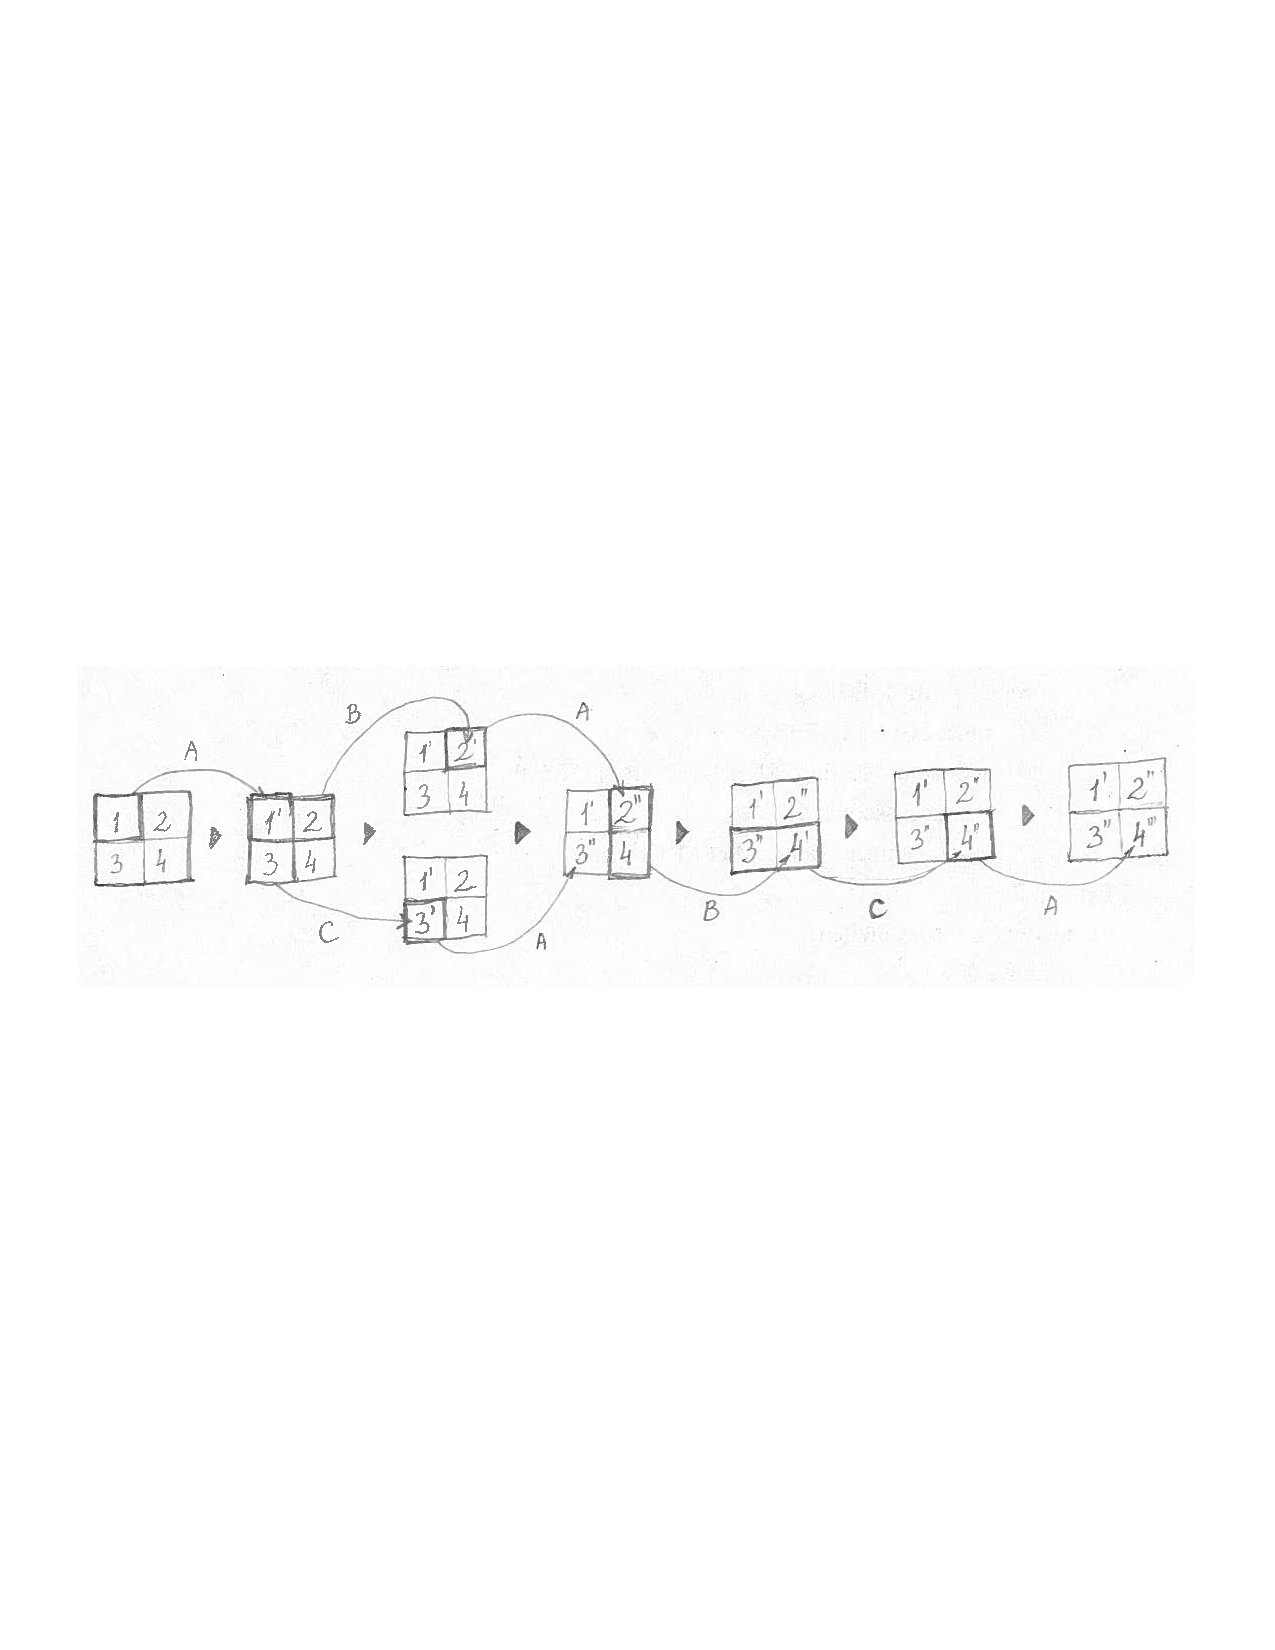
\includegraphics[width=.9\textwidth]{img/gap-stratify-A}
\end{center}
\caption{\label{evaluation:arbiter stratify A chain}}
\end{figure*}

\begin{comment}
This leads to the further stratified version shown in \Cref{evaluation:arbiter stratify A chain}.
The phases
$B$ and $C$ \eqref{intro:spec of B,C} are two more sub-problems that have to be addressed using the same slicing technique.
At first, it may seem that we have completed one task but created two; 
fortunately, $B$ and $C$ are much simpler instances\todo{for once, they are not recursive}
and are quite easy to develop.\todo{show this? Forget about this paragraph??}



\begin{center}$\vdots$
\end{center}

\end{comment}

\section{Related Work}
\label{related}

Classical work by Smith \etal~\cite{AI85/Smith} presents rule-based transformation, stringing it
tightly with program verification. This lay the foundation for semi-automatic programming~\cite{CPS91/Blaine,TSE90/Smith,TPHOLs96/Butler}.
More recently, a similar approach was introduced into Leon~\cite{OOPSLA13/Kneuss}, leveraging deductive
tools as a way to boost CEGIS, thereby covering more programs. Bellmania takes a dual approach, where
automated techniques based on SMT are leveraged to support and improve deductive synthesis.

Fiat~\cite{POPL15/Delaware} is another recent system that admits stepwise transformation of specifications
into programs via a refinement calculus. While Bellmania offloads proofs to automated solvers,
Fiat formalizes refinements using the Coq proof assistant. The user is then responsible of proving
the correctness of the derivation using a library of symbolic proof tactics.

Broadly speaking, the Bellmania system could have been implemented as a library on top of a framework
such as Coq or Why3~\cite{ESOP13/Filliatre} using binding to SMT solvers provided by these frameworks.
The decision not to do so was merely a design choice.

Our ``$\big/$'' operator can be compared to the separating disjunction ``$\ast$'' of Separation Logic~\cite{LICS02/Reynolds},
used to frame parts of the dynamic heap (which can be thought of as one large array),
in particular while checking that a program only accesses the parts allocated to it in its precondition.
While $\ast$ has the semantics of an existentially quantified predicate, Bellmania uses type qualifiers
to explicitly specify a formula defining each part. In this sense, it is more closely related to
Region Logic~\cite{ECOOP08/Banerjee}. These formulas make encoding in first-order logic straightforward,
and the use of Liquid Types allows for any number of dimensions and for decidable checking of domain inclusion
and disjointness.

\section{Conclusion}
\label{conc}

The examples in this paper show that a few well-placed tactics can cover a wide range
of program transformations. The introduction of solver-aided tactics allowed us to make
the library of tactics smaller, by enabling the design of higher-level, more generic
tactics. Their small number gives the hope that end-users with some mathematical background
will be able to use the system without the steep learning curve that is usually associated
with proof assistants. This can be a valuable tool for algorithms research.

Moreover, limiting the number of tactics shrinks the space in which to search for programs,
so that an additional level automation may be achieved via AI or ML methods. As more
developments are done by humans and collected in a database, those algorithms would become
more adept in predicting the next step of the construction.


\bibliographystyle{abbrvnat}
\bibliography{popl2016} % embed contents of popl2016.bbl for source submission

\end{document}
